\documentclass[12pt]{report}

\usepackage{csuf-thesis}
\usepackage{chicago}
\usepackage{breqn}
\usepackage{graphicx}
\usepackage{caption}
\usepackage{subcaption}
\usepackage[boxed]{algorithm2e}

\usepackage{listings}
\lstset{language=C++,basicstyle=\small}

\bibliographystyle{chicago}
\input{epsf}              % if you are using EPS figures

% Example of CSUF LaTeX style file
% SXW, Feb. 15, 2011

% First we need to initialize data for the thesis -
% Enter the author's name AS YOU WANT TO SEE IT TYPED
% REQUIRED
\author{Michael Robertson}

% Now we enter the title of the work in CAPITAL LETTERS
% This is bold centered on the titlepage.  There can be returns (\\) in
% this string if you have a long title. You must space it as a inverted pyramid.
% REQUIRED
\title{
LIGHTWAVE: AN INTERACTIVE \\
ESTIMATION OF INDIRECT \\
ILLUMINATION USING \\
WAVES OF LIGHT}

% Enter this degree.  This should be something in the following form:
%                       Master of Science
%                       Master of Art
% DEFAULT is Master of Science
\thisdegree{Master of Science}

% Enter the major of study.  This is used on the titlepage.
\major{Computer Science}

% Year degree is to be conferred
% DEFAULT is the current year and it is automatically generated using the system date
%\thesisyear{2011}

% Graduation Month - May or October
% DEFAULT is based on the time of year this document is processed
%\thesismonth{May}

% Now, enter your committee's information.  There three people on
% your committee.  The advisor is labeled as "Committee Chair"
% The other members are listed as "Committee Member"

\advisor{Dr. Michael Shafae}
% The advisor's department
\advisordept{Department of Computer Science}

\firstcomm{Dr. Kevin Wortman}
\firstcommdept{Department of Computer Science}

\secondcomm{Dr. Bin Cong}
\secondcommdept{Department of Computer Science}

% Are you going to obtain a copyright ?  Do you want a
% copyright page ?  If so, uncomment the following
%\yescopyright

% Do you have a copyright page but do not want one ?
% If so, uncomment the following
\nocopyright

% Now if we are attempting to fix only one included file, we can use
% the includeonly command.  Due to the way the style file works, the
% frontmatter will be generated each time (sorry :-( )
%\includeonly{chapter1, appendb}

%Let the document begin !
\begin{document}

% The following line generates a titlepage, copyright page (if requested)

\maketitle

% Now include the abstact. Make sure you have the file "abstract.tex" ready
\raggedright
\begin{abstract}

\paragraph{}
With the growth of computers and technology, so to has grown the desire to accurately recreate our world using computer graphics.  However, our world is very complex and in many ways beyond our comprehension.  Therefore, in order to perform this task, we must consider multiple disciplines and areas of research including physics, mathematics, optics, geology, and many more to at the very least approximate the world around us.  The applications of being able to do this are plentiful as well, including the use of graphics in entertainment such as movies and games, in science such as weather forecasts and simulations, in medicine with body scans, or used in architecture, design, and many other areas.  In order to recreate the world around us, an important task is to accurately recreate the way light travels and affects the objects we see.  Rendering lighting has been a heavily researched area since the 1970's and has gotten more sophisticated over the years.  Until recent developments in technology, realistic lighting of scenes has only been achievable offline taking seconds to hours or more to create a single image, however, due to advances in graphics technology, realistic lighting can be done in real-time.  An important aspect of realistic lighting involves the inclusion of indirect illumination.  However, to achieve a real-time rendering with indirect illumination, we must make trade offs between scientific accuracy and performance, but as will be discussed later, scientific accuracy may not be necessary after all.

\end{abstract}


% Generate a Table of Contents

\tableofcontents


% Generate a list of tables
% If you do not need a list of tables, comment this line

\listoftables

% Generate a list of figures (if you have any)
% If you do not need a list of figures, comment this line

\listoffigures

% Now include the acknowledegment. Make sure you have the file "acknowledgement.tex" ready
%\include{acknowledgement}

% There should be NO period at the end of the dedication. This is optional.
%\include{dedication}

% If the following line is uncommented, a new Table of Contents and list
% of figures will not be created and any "older" files of this type will
% be used.
%%\nofiles

% This command tells LaTeX that it is time to start the body of the
% work... it changes some format settings
\raggedright
\startbody

% You can include as many chapters as you have. Make sure you have the file "chapter1.tex" ready
\chapter{BACKGROUND}

\section{Light as a Particle and a Wave}
\paragraph{}
Before discussing current topics of research in the field of realistic light rendering in computer graphics, we first need a basic understanding of optics, a branch of physics that studies the behavior and properties of light.  Prior to the nineteenth century, light was regarded as a stream of particles and with this particle theory of light in mind, certain light phenomena such as refraction and reflection could be explained.  However in 1801, the first evidence of light acting as a wave was found when light rays were found to interfere with one another.  Later, in 1873, light was compared to a form of high-frequency electromagnetic wave.  In 1905, Einstein proposed a theory that explained the photoelectric effect (ejection of electrons from a metal surface when hit by light) that used the concept of quantization and stated that the energy of light waves is quantized in particles called photons. Quantization is the idea of constraining elements that are continuous into discrete sets. (Serway \& Jewett, 2004)  Therefore, light can have the behavior of a wave and a particle.  These findings are important to consider in our attempt to accurately depict light as it travels throughout a scene.  As will be discussed in the related work section, many lighting techniques use the idea that light consists of particles in order to simulate proper lighting conditions.  Some even have used the term photons such as in the lighting technique photon mapping.  This paper, however, will try to explore a hybrid approach that considers light as both a particle and as a wave.

\section{Terminology}
\paragraph{}
Lastly, before jumping into the related work section, we must cover some basic terminology used in current papers covering lighting in computer graphics.  Lighting or illumination, is broken down into different components.  Direct illumination is the rendering of a scene as it would appear if the light rays from the light sources terminated or ended at the first surface they hit.  Scenes made with this type of illumination are high performance but low realism due to attributes such as hard shadows, no reflection or refraction, and the fact that only surfaces in view of the light source are illuminated with everything else black.  In order to make the scene more realistic, we need to add indirect illumination.  Indirect illumination considers the behavior of light after it hits a surface.  It features the reflection and refraction of light and produces realistic scenes depending on the extent of indirect illumination captured.  It illuminates the surfaces that are not directly visible by the light source such as behind another object.  Light can be interpreted as bouncing through a room infinitely until the energy of the light reaches zero and is completely absorbed by the surfaces in the room.  Noting this, indirect illumination can be recursively calculated to infinity and therefore can be expressed using a Neumann series where we calculate the sum of light hitting a surface point due to the reflection of light from other surfaces $n$-times with $n$ approaching infinity.  Then the performance of calculating the indirect illumination depends on how large $n$ is along with other factors discussed later, but is typically much slower than calculating direct illumination.  Once we have direct illumination and indirect illumination calculated, we can say that we have the global illumination of the scene.  This paper's goal is to exploit the high performance of direct illumination by trying to approximate the indirect illumination of a single light source by using the direct illumination of multiple virtual light sources.

\chapter{PREVIOUS WORK} \label{sec:prevwork}

\section{Real-Time Versus Offline Rendering Techniques}
\paragraph{}
Rendering techniques can be broken down into two distinct categories: real-time and offline.  Offline rendering techniques require anywhere from seconds to many hours to render a single image.  Current offline rendering techniques are able to render ultra-realistic images that take into account many light sources as well as many types of lighting principles such as reflection, refraction, sub-surface light scattering, and others in very complex scenes consisting of millions of triangles and at high resolutions.  Real-time rendering techniques render images at a fast enough rate to support multiple frames a second and vary greatly in approach.  These techniques can be broken down into dynamic and static.  Dynamic scenes allow a user to interact with the scene by actively moving the geometry, the camera, or the light source whereas static scenes do not.  As opposed to offline techniques, real-time techniques have to make sacrifices and therefore can't be as scientifically accurate as offline techniques.  The goal of this paper is to create a real-time technique that supports a fully dynamic scene.  Regardless of whether the technique is offline or real-time, the algorithm used can trace it's roots back to a single equation, \textit{The Rendering Equation}.

\section{The Rendering Equation} \label{sec:render}
\paragraph{}
When discussing light transport in computer graphics, the most significant paper is \textit{The Rendering Equation} by Kajiya (1986).  In it, Kajiya presents an equation that generalizes most rendering algorithms.  Such a statement can be confirmed by the fact that all rendering equations try to recreate the scattering of light off of different types of surfaces and materials.  The rendering equation is an integral that is adapted from the study of radiative heat transfer for use in computer graphics with an aim at balancing the energy flow between surfaces.  The equation, however, is still an approximation because it does not take into account diffraction and it assumes that the space between objects, such as air, is of homogeneous refractive index meaning that light won't refract due to the particles in the air.

\begin{equation}
I(x,x') = g(x,x')[\epsilon(x,x')+\int_{S} \rho(x,x',x'')I(x',x'')dx''] \label{eqn:render}
\end{equation}

\paragraph{}
The rendering equation is broken down into 4 parts.  First, $I(x,x')$ is the intensity of light or energy of radiation passing from point $x'$ to point $x$ measured in energy of radiation per unit time per unit area.  Second, the geometry term, $g(x,x')$, indicates the occlusion of objects by other objects.  This term is either $0$, if $x$ and $x'$ are not visible from one another, or $1/r^2$ where $r$ is the distance between $x$ and $x'$ if $x$ and $x'$ are visible from one another.  Third, the emittance term, $\epsilon(x,x')$, measures the energy emitted from point $x'$ that reaches point $x$.  Lastly, the scattering term, $\rho(x,x',x'')$, is the intensity of energy scattered by a surface point $x'$ that originated from point $x''$ and then ends at point $x$.  As mentioned in the previous section, global illumination can be calculated using the Neumann series.  A Neumann series is a mathematical series of the form:
\begin{equation}
\sum_{k=0}^{\infty}T^k \label{eqn:neumann}
\end{equation}

where $T$ is an operator and therefore $T^k$ is a notation for $k$ consecutive operations of operator $T$. 

\paragraph{}
Furthermore, the rendering equation can also be approximated using the Neumann series.  This is done by rewriting the rendering equation above (\ref{eqn:render}) as:
\begin{equation}
I = g\epsilon +gMI \label{eqn:render2}
\end{equation}
where $M$ is the linear operator given by the integral in the rendering equation.  Next, we rewrite equation \ref{eqn:render2} as:
\begin{equation}
(1-gM)I = g\epsilon \label{eqn:render3}
\end{equation}
so that we can invert it to get:
\begin{equation}
I = g\epsilon + gMg\epsilon + gMgMg\epsilon +g(Mg)^3\epsilon + ... \label{eqn:render4}
\end{equation}
Equation \ref{eqn:render4} is a Neumann series of the form:
\begin{equation}
I = g\epsilon\sum_{k=0}^{\infty}(Mg)^k \label{eqn:render5}
\end{equation}
Equation \ref{eqn:render5} indicates that the rendering equation (equation \ref{eqn:render}) is the final intensity of radiation transfer as a sum of a direct term, a once scattered term, a twice scattered term, and so on.  Therefore, as mentioned in the previous chapter, indirect illumination can be calculated by summing the light incident on a surface due to the reflection of light $n$-times as $n$ approaches infinity.  The more scattered terms we include in the calculation, the better the approximation will be but with worse performance.  Therefore, in real-time applications, this needs to be avoided.  

\paragraph{}
Next, we show how the rendering equation can be seen has a generalization of most rendering algorithms, but first we must cover some other rendering techniques beginning with offline rendering techniques.

\section{Offline Rendering Techniques}
\paragraph{}
Key examples of offline rendering techniques are ray tracing, radiosity, and photon maps.  We begin with ray tracing.

\subsection{Ray Tracing}

\begin{figure}[h!]
  \centering
    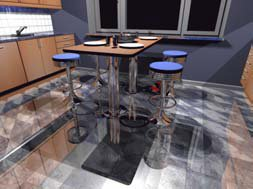
\includegraphics[width=0.5\textwidth]{raytraceSample.jpg}
  \caption{Image produced using ray tracing.}
	\label{fig:raytraceSample}
\end{figure}

\paragraph{}
Ray tracing is a technique for rendering an image of a three-dimensional scene by casting rays from a camera positioned somewhere in the scene.  Each ray is shot into the scene and it registers the first surface it hits.  From this surface point, additional rays go to each of the light sources to determine visibility to render shadows as well as to other surfaces to render reflections as shown in figure \ref{fig:raytraceCalc} from Ward, Rubinstein, and Clear (1988).  These rays can also be used to calculate other lighting phenomena such as refractions.

\begin{figure}[h!]
  \centering
    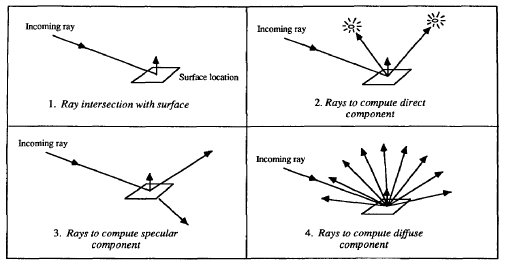
\includegraphics[width=1.0\textwidth]{raytraceCalc.jpg}
  \caption{Steps of ray tracing.}
	\label{fig:raytraceCalc}
\end{figure}

\paragraph{}
The rays from the camera can be cast into the scene using different sampling patterns and techniques such as one ray per pixel or many rays per pixel.  Also, the rays can be cast through the center of each pixel or through the use of stochastic sampling can be cast through non-uniformly spaced locations in each pixel to avoid aliasing artifacts or jaggies as shown in figures \ref{fig:sampling} and \ref{fig:jaggies} from Reeves, Salesin, and Cook (1987).

\begin{figure}[h!]
  \centering
    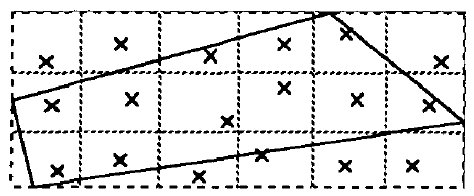
\includegraphics[width=0.5\textwidth]{sampling.jpg}
  \caption{Sampling non-uniformly spaced locations in each pixel.}
	\label{fig:sampling}
\end{figure}

\begin{figure}[h!]
  \centering
    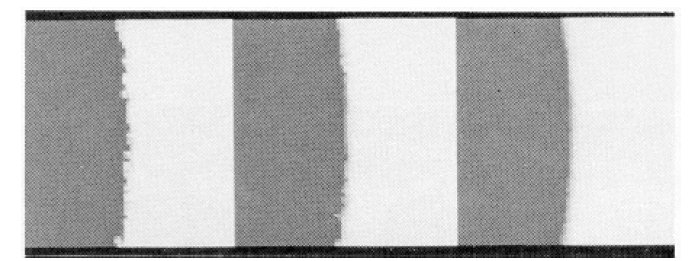
\includegraphics[width=0.5\textwidth]{jaggies.jpg}
  \caption{Image of aliasing artifacts known as jaggies. Better sampling results in softer edges.}
	\label{fig:jaggies}
\end{figure}

\paragraph{}
Ray tracing is able to recreate ultra-realistic scenes such as figure \ref{fig:raytraceSample} from Wald, Benthin, and Slusallek (2003) but at a high cost.  Examples of ray tracing techniques can be seen in the work of Whitted (1980), Cook (1986), and Ward et al. (1988).  With adaptations to ray tracing techniques and advances in technology, there now exist some interactive ray-tracing techniques mentioned in section \ref{sec:RT}.

\paragraph{}
Ray tracing can also be related to the rendering equation.  Whitted (1980) describes a new approximation for ray tracing by rewriting the Phong illumination model in order to improve the quality of specular reflections.  The Phong illumination model is a way of calculating lighting on a surface through the combination of three components: ambient, diffuse, and specular.  Diffuse is the reflection of light from rough surfaces, specular is the reflection of light on shiny surfaces, and the ambient component accounts for the amount of light that is scattered throughout the scene.  The ambient term is most similar to indirect lighting, but is a user-specified constant amount distributed uniformly throughout the scene to avoid any actual calculations.  The improved model from Whitted (1980) is written:
\begin{equation}
I = I_{a} + k_{d}\sum_{j=1}^{j=ls}(\bar{N}\cdot\bar{L}_{j})+k_{s}S + k_{t}T \label{eqn:raytrace1}
\end{equation}

where $S$ is the intensity of light incident from the specular reflection direction, $k_{t}$ is the transmission coefficient, and $T$ is the intensity of light from the transmitted light direction. $k_{s}$ and $k_{t}$ are coefficients that are to be used to try to accurately model the Fresnel reflection law, which is an equation that describes how light behaves when moving from one medium to another with a different refractive index.  Equation \ref{eqn:raytrace1} is in the form of equation \ref{eqn:render4} from Kajiya (1986) with $M$ as the sum of the reflection and refraction terms as well as the diffuse component. Then the term $g$ considers shadows and the ambient term can be approximated by the $\epsilon$ term.  Lastly, $M$ is approximated by summing over all the light sources rather than using integration.

\subsection{Radiosity}

\begin{figure}[h!]
  \centering
    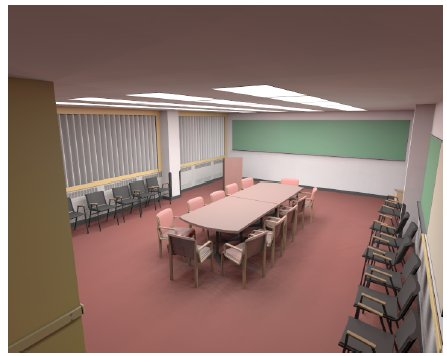
\includegraphics[width=0.5\textwidth]{radiositySample.jpg}
  \caption{Image rendered using radiosity.}
	\label{fig:radiositySample}
\end{figure}

\paragraph{}
Radiosity is a type of rendering technique that was adapted for use in computer graphics from the thermal engineering field.  The method is based on the fundamental Law of Conservation of Energy within a closed area.  This law states that energy can neither be created nor destroyed and that the energy in this closed area is to remain constant over time.  It provides a global solution for the intensity of light incident on each surface by solving a system of linear equations that describes the transfer of energy between each surface in the scene.  Examples of radiosity can be found in the works of Immel, Cohen, and Greenberg (1986) and Goral, Torrance, Greenberg, and Battalie (1984) and shown in figure \ref{fig:radiositySample} from Keller (1997).

\paragraph{}
Radiosity is a natural extension from the rendering equation (equation \ref{eqn:render}) since its focus is on balancing the flow of energy.  The only difference is that radiosity makes assumptions about the reflectance characteristics of the surface material.  The radiosity in the scene is found by taking the hemispherical integral of the energy leaving the surface called flux seen in figure \ref{fig:radiosityCalc1} from Immel et al. (1986).  This can be found using the following equation from Goral et al. (1984):
\begin{equation}
B_{j} = E_{j} + \rho_{j}H_{j} \label{eqn:radiosity1}
\end{equation}

where $B_{j}$ is the rate of energy leaving the surface $j$ measured in energy per unit time per unit area, $E_{j}$ is the rate of direct energy emission,  $\rho_{j}$ is the reflectivity of surface $j$, and $H_{j}$ is the incident radiant energy arriving at surface $j$ per unit time per unit area as depicted in figure \ref{fig:radiosityCalc2} from Goral et al. (1984).

\begin{figure}[h!]
  \centering
    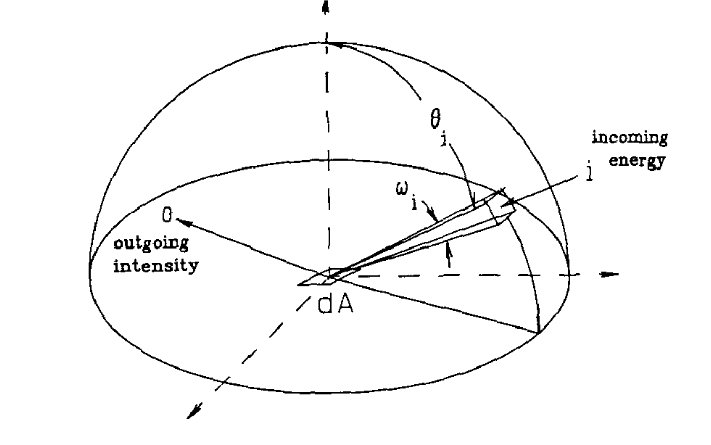
\includegraphics[width=0.75\textwidth]{radiosityCalc1.jpg}
  \caption{Hemispherical integral of the energy leaving the surface.}
	\label{fig:radiosityCalc1}
\end{figure}

\begin{figure}[h!]
  \centering
    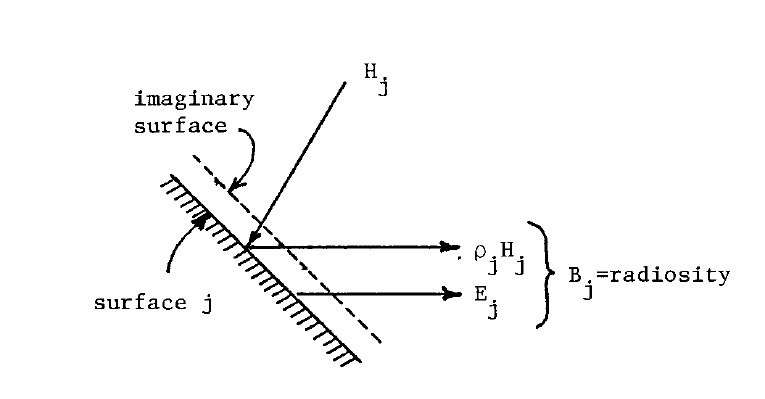
\includegraphics[width=0.75\textwidth]{radiosityCalc2.jpg}
  \caption{Illustration of equation \ref{eqn:radiosity1}.}
	\label{fig:radiosityCalc2}
\end{figure}

\paragraph{}
Equation \ref{eqn:radiosity1} can be derived using our rendering equation (equation \ref{eqn:render}) by Kajiya (1986) by integrating over all surfaces in the scene to calculate the hemispherical quantities, calculating the contribution of the emittance and reflectance terms by checking for occlusions, and by using those calculations the rendering equation becomes:
\begin{equation}
dB(x') = \pi[\epsilon_{0} + \rho_{0}H(x')]dx' \label{eqn:radiosity2}
\end{equation}

where $\epsilon_{0}$ is the hemispherical emittance of the surface element $dx'$, $\rho_{0}$ comes from the reflectance term, and $H$ is the hemispherical incident energy per unit time per unit area.  This adaptation of the rendering equation (equation \ref{eqn:radiosity2}) is the same as the radiosity equation shown above (equation \ref{eqn:radiosity1}).

\subsection{Photon Maps}

\begin{figure}[h!]
  \centering
    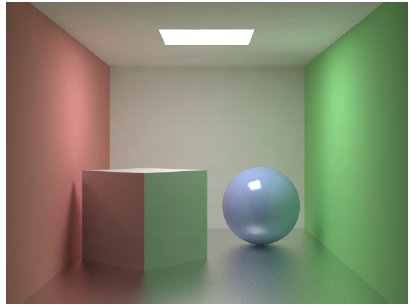
\includegraphics[width=0.5\textwidth]{photonSample.jpg}
  \caption{Image rendered using photon maps.}
	\label{fig:photonSample}
\end{figure}

\paragraph{}
Photon maps originally introduced by Jensen (1996) is a two pass global illumination method that produces images such as that seen in figure \ref{fig:photonSample}.  As mentioned in the Background section, Einstein coined the term photon for the particles present in the energy of light waves.  In the method of photon mapping, the term photon is used in a similar context.  The first pass of the method consists of making two photon maps by emitting packets of energy called photons from the light sources and storing where they hit surfaces in the scene as seen in figure \ref{fig:photonCalc}.  The second pass of the method calls for the use of a distribution ray tracer that is optimized using the data gathered in the photon maps.  Photon maps are able to render complex lighting principles such as the caustics seen in figure \ref{fig:photonCaustics}.

\begin{figure}[h!]
  \centering
    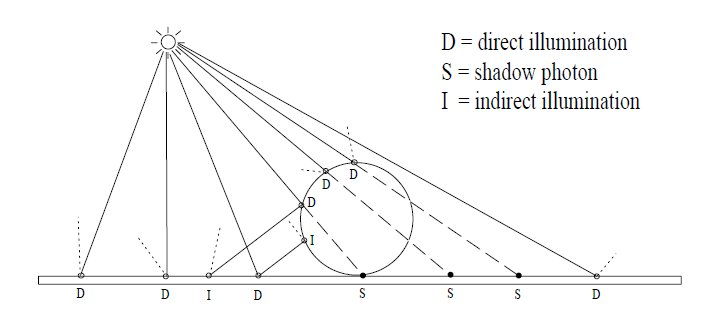
\includegraphics[width=1.0\textwidth]{photonCalc.jpg}
  \caption{Process of casting photons into the scene.}
	\label{fig:photonCalc}
\end{figure}

\begin{figure}[h!]
  \centering
    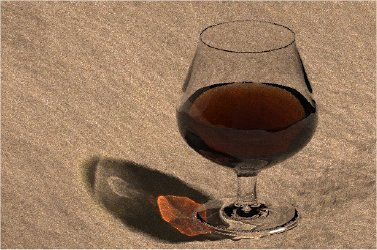
\includegraphics[width=0.5\textwidth]{photonCaustics.jpg}
  \caption{Example of caustics.}
	\label{fig:photonCaustics}
\end{figure}

\paragraph{}
Photon maps are an extension to the rendering equation (equation \ref{eqn:render}) as well.  During the second pass of the method, the scene is rendered by calculating the radiance by tracing a ray from the eye through the pixel and into the scene using ray tracing, and the radiance is computed at the first surface that the ray hits.  The surface radiance leaving the point of intersection $x$ in some direction is computed using this equation from Jensen (1996):
\begin{equation}
L_{s}(x,\psi_{r} = L_{e}(x,\psi_{r} + \int_{\Omega}(f_{r}(x,\psi_{i};\psi_{r})L_{i}(x,\psi_{i})\cos(\theta_{i})d\omega_{i}) \label{eqn:photon1}
\end{equation}

where $L_{e}$ is the radiance emitted by the surface, $L_{i}$ is the incoming radiance in the direction $\psi_{i}$, and $f_{r}$ is the BRDF or bidirectional reflectance distribution function, which is a four-dimensional function that describes how light is reflected at a surface point.  Lastly, $\Omega$ is the sphere of incoming directions.  This can be broken down into a sum of four components:
\begin{align}
  &\begin{aligned} \label{eqn:photon2}
    L_{r} &=  \int_{\Omega} (f_{r}L_{i,l}\cos(\theta_{i})d\omega_{i}) + \int_{\Omega}(f_{r,s}(L_{i,c}+L_{i,d})\cos(\theta_{i})d\omega_{i})\\
      &\qquad + \int_{\Omega} (f_{r,d}L_{i,c}\cos(\theta_{i})d\omega_{i}) +  \int_{\Omega}(f_{r,d}L_{i,d}\cos(\theta_{i})d\omega_{i}
  \end{aligned}
\end{align}

where the first term of equation \ref{eqn:photon2} is the contribution by direct illumination, the second term is the contribution by specular reflection, the third term is the contribution by caustics, and the fourth term is the contribution by soft indirect illumination.  Both equations \ref{eqn:photon1} and \ref{eqn:photon2} are direct adaptations from the rendering equation in as introduced by Kajiya (1986) (equation \ref{eqn:render}).

\subsection{Other Offline Rendering Techniques} \label{sec:otheroffline}
\paragraph{}
Many recent offline techniques have been influenced by real-time techniques most notably the idea of using virtual point lights or VPL's as introduced in \textit{Instant Radiosity} by Keller (1997).  This technique will be discussed in detail in the real-time rendering techniques section, but the main idea is that we can render indirect light through the use of a set of VPL's where we accumulate the contributions of each of these lights in multiple rendering passes.  This technique is used for rendering illumination from area lights, high dynamic range (HDR) environment maps or sun/sky models, single/multiple subsurface light scattering in participating media, and most importantly for our purposes indirect illumination.  For offline purposes, techniques typically call for the use of millions of VPL's to achieve higher quality renderings, however, many techniques attempt to mitigate the cost of using such a large number of lights.

\paragraph{}
\underline{Virtual Point Lights}: In \textit{Lightcuts: A Scalable Approach to Illumination} by Walter et al. (2005), it is discussed that when using many lights, as in the VPL method, the cost to render the scene scales linearly with the number of lights used.  This limits the number of VPL's we can use without serious performance impact.  Therefore, the Lightcuts method is introduced as a way to reduce the rendering cost of using VPL methods by making it “strongly sub-linear” with the number of lights used without noticeable impact on quality.  Using this method, hundreds of thousands of point lights can be accurately rendered using only a few hundred shadow rays.  Lightcuts does this by clustering a group of VPL's together to form a single brighter light thereby reducing the cost of rendering the group of lights present in the cluster group to a single light.  This is done by using a global light tree which is a binary tree that has individual VPL's as the leaves and interior nodes as the light clusters that contain the individual lights below it in the tree as seen in figure \ref{fig:lightTree} shown in Walter et al. (2005).  A cut of this tree then is ``a set of nodes such that every path from the root of the tree to a leaf will contain exactly one node from the cut'' and will represent a valid clustering of the lights.  This approach was further advanced in \textit{Multidimensional Lightcuts} by Walter, Arbree, Bala, and Greenberg (2006) for use with visual effects such as motion blur, participating media, depth of field, and spatial anti-aliasing in complex scenes and used again in \textit{Bidirectional Lightcuts} by Walter, Khungurn, and Bala (2012) to support low noise rendering of complicated scenes with glossy surfaces, subsurface BSSRDF's, and anisotropic volumetric models.

\begin{figure}[h!]
  \centering
    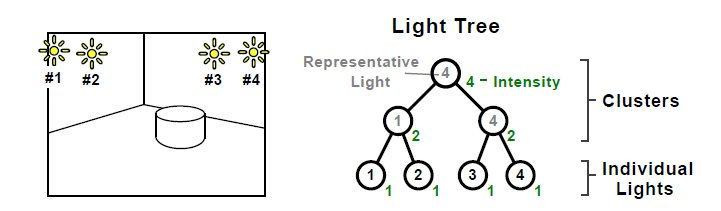
\includegraphics[width=1.0\textwidth]{lightTree.jpg}
  \caption{Example of a light tree.}
	\label{fig:lightTree}
\end{figure}

\paragraph{}
\underline{Matrix Sampling}: Another adaption of the VPL method in offline rendering techniques is with the use of mathematical matrix sampling to reduce the rendering cost.  In \textit{Matrix Row-Column Sampling for the Many-Light Problem} by Hašan, Pellacini, and Bala (2007), it is shown that many point lights can be seen as a large matrix of sample-light interactions.  The final image is then the sum of all of the columns of the matrix.  Therefore, by sampling this matrix and using a small number of the rows and columns, we can approximate the final image at a fraction of the rendering cost.  The matrix used in this technique is comprised of the columns representing all of the surface points to be lit by each light and each row being comprised of all of the lights in the scene.  Then it can often be shown that this matrix is of low rank meaning that the row and/or columns of the matrix can be linearly combined to form a smaller matrix that would approximate the original larger matrix.  Therefore, this method approaches the problem in a similar way as Lightcuts, but instead of using a tree, we use a matrix.  This method is comprised of four primary steps.  First, we sample $r$ randomly selected rows using shadow maps on the GPU.  Shadow maps will be discussed in the next section.  Next, we partition the reduced columns into clusters on the CPU.  Third, we pick a representative from each cluster to be scaled appropriately to account for the entire cluster on the CPU.  Last, we accumulate each of these representatives using shadows maps on the GPU.  By using this method, the render time of shading $m$ surface points using $n$ VPL's is reduced from $O(mn)$ to $O(m+n)$ as seen in figure \ref{fig:matrixSampling} by Hašan et al. (2007).  Additionally, \textit{LightSlice: Matrix Slice Sampling for the Many-Lights Problem} by Ou and Pellacini (2011) uses a similar approach as in Hašan et al. (2007) and Walter et al. (2005), but found that neither technique optimally exploits the structure of the matrices in scenes with large environments and complex lighting so some modifications were made to reduce render time and improved overall quality.

\begin{figure}[h!]
  \centering
    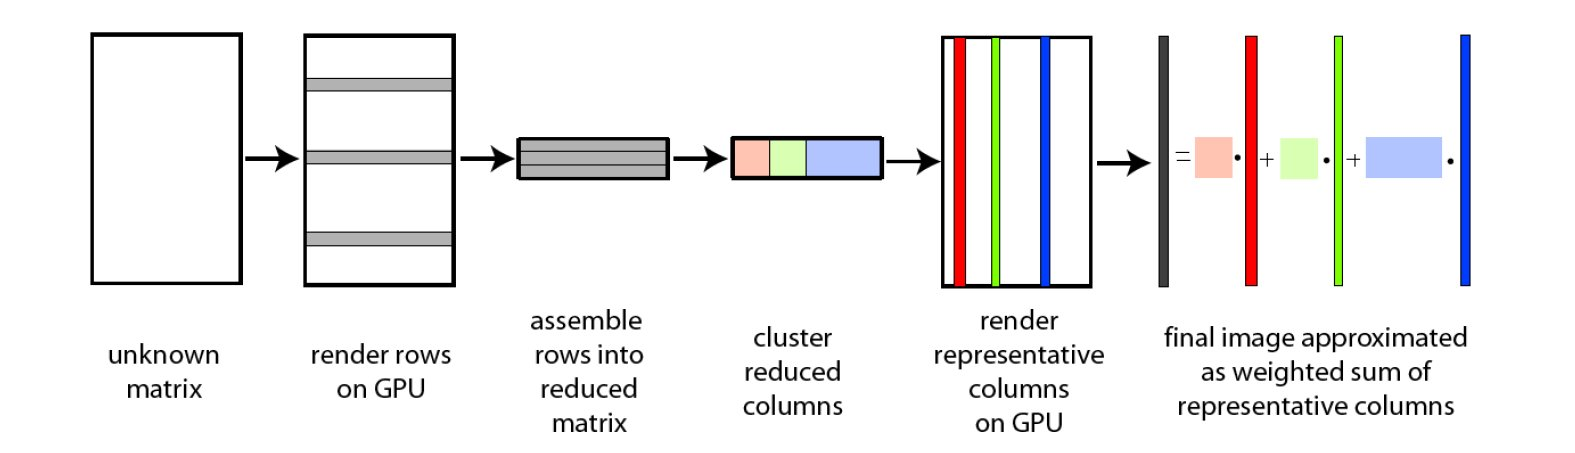
\includegraphics[width=1.0\textwidth]{matrixSampling.jpg}
  \caption{Overview of matrix sampling algorithm.}
	\label{fig:matrixSampling}
\end{figure}

\paragraph{}
\underline{Shadow Maps}: Shadow maps are textures that are typically used to render shadows, but as shown in the real-time rendering techniques section, they have additional uses.  They are created in a render pass where the view of the scene is computed from the light source's point of view and the distances from the light to the nearest surface for each pixel is stored in this texture or buffer to be used for comparisons when rendering the scene from the camera's point of view to determine whether a surface point is in shadow as presented by Williams (1978) and by Reeves, Salesin, and Cook (1987).  See figures \ref{fig:shadowMap1} and \ref{fig:shadowMap2} by Dachsbacher and Stamminger (2005)for an image of a shadow map and the resulting final image, respectively.  Further discussion on shadow maps will be done in the real-time rendering techniques section as well as in the implementation section.
\begin{figure}[h!]
  \centering
    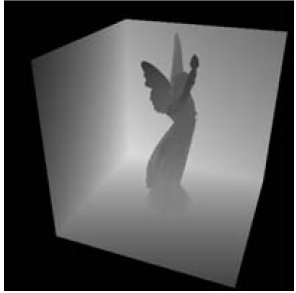
\includegraphics[width=0.5\textwidth]{shadowMap1.jpg}
  \caption{Image of a shadow map. Scene is from the view of the light source.}
	\label{fig:shadowMap1}
\end{figure}
\begin{figure}[h!]
  \centering
    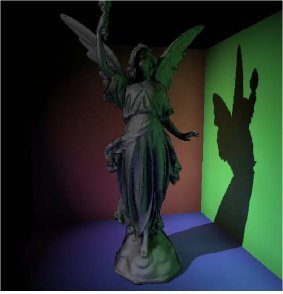
\includegraphics[width=0.5\textwidth]{shadowMap2.jpg}
  \caption{Resulting image using the shadow map from \ref{fig:shadowMap1}.}
	\label{fig:shadowMap2}
\end{figure}

\paragraph{}
\underline{Virtual Ray Lights}: Lastly, Novák, Nowrouzezahrai, Dachsbacher, and Jarosz (2012) describes a technique to render scenes with single/multiple light scattering in participating media in \textit{Virtual Ray Lights for Rendering Scenes with Participating Media}.  The technique modifies the idea of using VPL's by instead using virtual ray lights or VRL's inside the participating media.  So instead of evaluating each VPL at discrete locations, we calculate the contribution of each VRL with an efficient Monte Carlo sampling technique.  Monte Carlo sampling involves the use of randomly selecting a point based off a probability distribution and is often used for sampling in a wide variety of techniques.  The reason for using VRL's over VPL's is that VPL's can be negatively affected by singularities in the scene.  A singularity is when a given value or location is undefined in our equation.  For example, the equation $1/x$ is undefined for $x=0$.  Singularities are common along boundaries of walls as seen in figure \ref{fig:singularity} by Dachsbacher and Stamminger (2005).  These singularities can cause artifacts in the scene such as spikes of high intensity which can be eliminated through the use of clamping or blurring.  But by using a VRL, we compute the contribution of the light by distributing the energy over a line segment reducing singularities as shown in figure \ref{fig:vrl} by Novák et al. (2012).  In this case, instead of having spikes of high intensity, we have a uniform noise distributed evenly over the image which would be more pleasing to the eye.

\begin{figure}[h!]
  \centering
    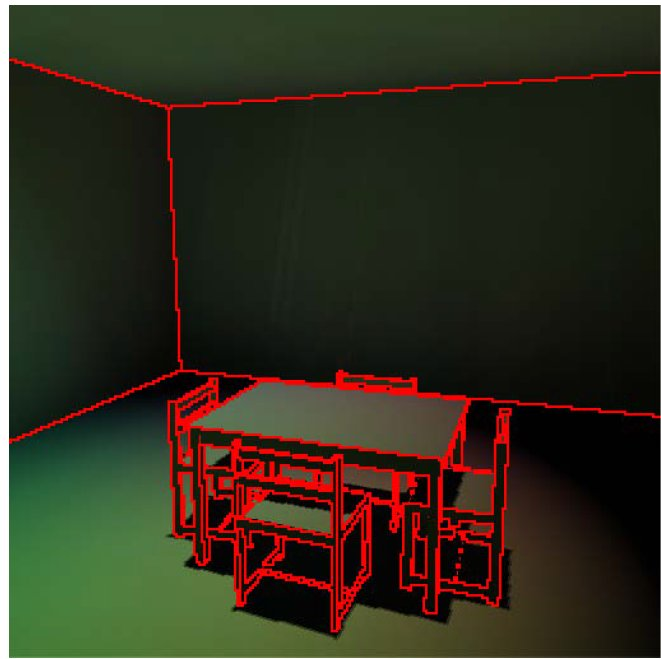
\includegraphics[width=0.5\textwidth]{singularity.jpg}
  \caption{Common locations where singularities exist.}
	\label{fig:singularity}
\end{figure}

\begin{figure}[h!]
  \centering
    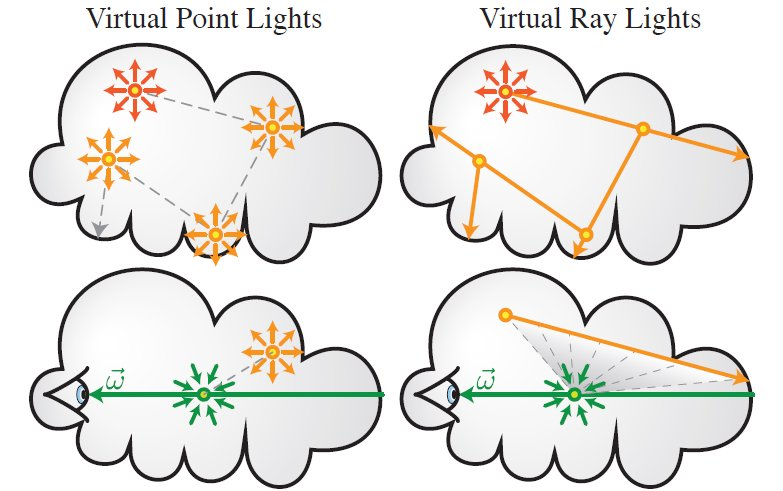
\includegraphics[width=1.0\textwidth]{vrl.jpg}
  \caption{VRL versus VPL.}
	\label{fig:vrl}
\end{figure}

\section{Real-Time Rendering Techniques} \label{sec:RT}
\paragraph{}
With the advancement of technology and the expanded use of the GPU, many offline rendering techniques have been adapted to work on the GPU to run in real-time usually by making trade offs and approximations.  This includes interactive ray tracing by Wald, Kollig, Benthin, Keller, and Slusallek (2002), approximate ray tracing on the GPU by Szirmay-Kalos, Aszodi, Lazanyi, and Premecz (2005), image space photon mapping by McGuire and Luebke (2009), and \textit{Instant Radiosity} by Keller (1997).  The most significant advancement coming from the idea of virtual point lights as in \textit{Instant Radiosity}.

\subsection{\textit{Instant Radiosity}} \label{sec:instantradiosity}
\paragraph{}
As discussed in prior sections, \textit{Instant Radiosity} introduces the technique of approximating indirect illumination by using virtual points lights where each individual light acts independently as a producer of indirect illumination and behaves like a normal point light source.  In the original technique, these VPL's are generated using a quasi-random walk technique created at the hit points of the photons as they are traced into the scene from the primary light source seen in figure \ref{fig:vrl}.  The contributions of these VPL's are then summed through the use of multiple rendering passes.  This implementation had a few limitations such as requiring many rendering passes to support dynamic objects or lights as well as being limited to simple environments due to the high cost of computing shadows for each of the VPL's.  These shadows had to be computed by using shadow volumes or shadow maps and were the bottleneck of the technique.  There were also issues with low sampling rates which would result in weak singularities when the VPL got increasingly close to the illuminated surface point and each VPL had a high influence or contribution on the overall color of the final image.  Also, temporal flickering could be seen if there were not enough VPL's being used.  Despite these issues, real-time performance was attainable in 1997 through the use of this technique.

\subsection{Adaptations of \textit{Instant Radiosity}}
\paragraph{}
In addition to the offline techniques already mentioned which adapted the idea of using VPL's for the offline rendering of a variety of lighting phenomena, many real-time techniques also adapted the use of VPL's.

\paragraph{}
\underline{Shadow Map Alterations}: As teased in section \ref{sec:otheroffline}, many real-time rendering techniques expanded the use of shadow maps beyond just creating shadows.  \textit{Translucent Shadow Maps} by Dachsbacher and Stamminger (2003) extended the binary shadow map look-up to a shadow map filter to assist in the implementation of real-time sub-surface scattering.  Translucent Shadow Maps extend shadow maps by having additional information stored such as depth and incident light information.  Therefore, each pixel in the Translucent Shadow Map stores the 3D position of the surface sample, the irradiance entering the object at that sample, and the surface normal.  Although this implementation was for sub-surface scattering, it would lead to a development in rendering indirect illumination as well.

\paragraph{}
From this idea of extending shadow maps came further developments in \textit{Reflective Shadow Maps} abbreviated RSM by Dachsbacher and Stamminger (2005).  This technique extended a shadow map such that each pixel in the shadow map would be thought of as an indirect light source.  The reflective shadow map then stored information such as depth value, world space position, normal, and reflected radiant flux shown in figure \ref{fig:RSM} by Dachsbacher and Stamminger (2005).  With all this information available, we can then approximately calculate the indirect irradiance at a surface point by summing the illumination due to all pixel lights as seen in equations \ref{eqn:RSM1} and \ref{eqn:RSM2}.
\begin{equation}
E_{p} (x,n) = \Phi_{p} {max(0, n_{p} \cdot (x-x_{p})) max(0, n_{p} \cdot (x_{p} - x))  } \div {\| x-x_{p} \|^{4} } \label{eqn:RSM1}
\end{equation}
\begin{equation}
E(x,n) = \sum_{pixels p} E_{p}(x,n) \label{eqn:RSM2}
\end{equation}

\begin{figure}
		\centering
        \begin{subfigure}[b]{0.4\textwidth}
                \centering
                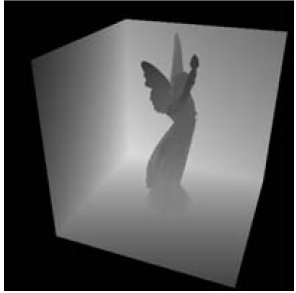
\includegraphics[width=\textwidth]{shadowMap1.jpg}
                \caption{Depth Values.}
                \label{fig:RSM0}
        \end{subfigure}
        \begin{subfigure}[b]{0.4\textwidth}
				\centering
                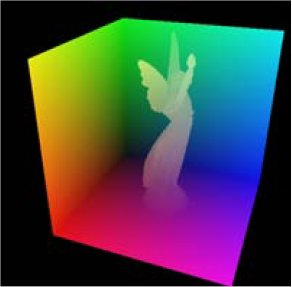
\includegraphics[width=\textwidth]{RSM1.jpg}
                \caption{World Space Positions.}
                \label{fig:RSM1}
        \end{subfigure}
        \begin{subfigure}[b]{0.4\textwidth}
        		\centering
                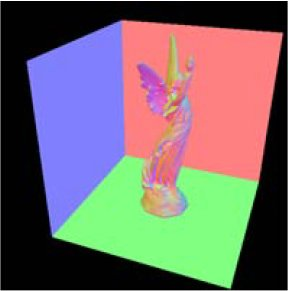
\includegraphics[width=\textwidth]{RSM2.jpg}
                \caption{Normal Values.}
                \label{fig:RSM2}
        \end{subfigure}
        \begin{subfigure}[b]{0.4\textwidth}
        		\centering
                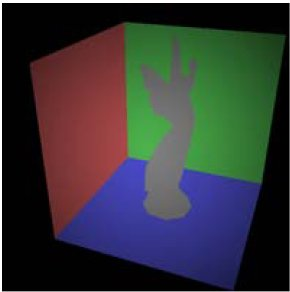
\includegraphics[width=\textwidth]{RSM3.jpg}
                \caption{Reflected Radiant Flux.}
                \label{fig:RSM3}
        \end{subfigure}
        \caption{Data stored in the RSM.}\label{fig:RSM}
\end{figure}

where $x$ is the surface point, $n$ is the normal at $x$, $n_{p}$ and $x_{p}$ is the pixel light normal and position, and $\Phi_{p}$ is the reflected radiant flux of the visible surface point as shown in figure \ref{fig:RSMcalc} by Dachsbacher and Stamminger (2005).  This technique had the same singularity issue near the boundary of two adjoining walls shown earlier in figure \ref{fig:singularity}.  Other limitations includes having to ignore occlusion and visibility for the indirect light sources as well as having to restrict the number of VPL's to around 400 meaning that sampling had to be done to chose the 400 best VPL's.  Also, screen-space interpolation had to be performed by computing the indirect illumination using a low-resolution shadow map and interpolating using multiple low-res samples.  With these restrictions in play, this technique renders approximate indirect illumination for dynamic scenes.

\begin{figure}[h!]
  \centering
    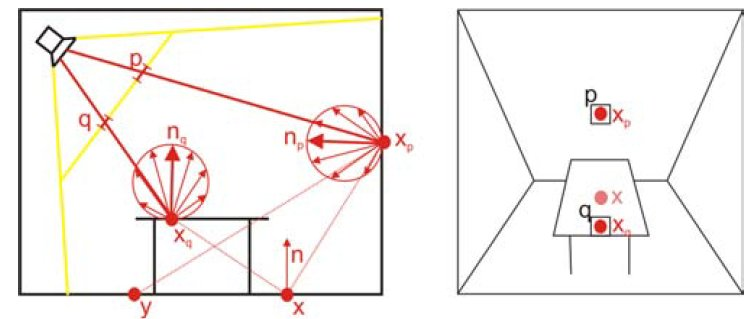
\includegraphics[width=1.0\textwidth]{RSMcalc.jpg}
  \caption{Illustration of equations \ref{eqn:RSM1} and \ref{eqn:RSM2}.}
	\label{fig:RSMcalc}
\end{figure}

\paragraph{}
Reflective shadow maps were then used in many other real-time rendering techniques that followed.  This included \textit{Splatting Indirect Illumination} by Dachsbacher and Stamminger (2006) which rendered the VPL's contributions through a splatting technique in a deferred shading process which reduced the effect of scene complexity on the rendering time.  It also allowed for efficient rendering of caustics and reduced scene artifacts.

\paragraph{}
Additionally, RSM's are used in other applications such as indirect illumination for area light sources as in \textit{Direct Illumination from Dynamic Area Lights With Visibility} by Nichols, Penmatsa, and Wyman (2010).  Here we use RSM's to generate VPL's, but add visibility to the technique by computing occlusion by marching rays towards each VPL through a voxel buffer.  The technique then checks the visibility for each VPL and adds in its illumination provided the VPL is visible.

\paragraph{}
\textit{Imperfect Shadow Maps for Efficient Computation of Indirect Illumination} by Ritschel et al. (2008) altered shadow maps for their purposes by making them imperfect shadow maps or ISM's.  These ISM's were low resolution shadow maps with a simplified point-representation of the scene such that some of the depth values could be incorrect.  This simplified scene is done by approximating the 3D scene by a set of points with a near uniform density which is then used to create an ISM.  The point-based representation of the geometry is used to allow the creation of hundreds of ISM's in parallel in a single pass to support dynamic scenes.  These hundreds of ISM's are stored in a single large texture and are used for approximate visibility for the hundreds or thousands of VPL's used for indirect illumination.  These VPL's are generated through the use of RSM's.  ISM's can also be built on top of reflective shadow maps to create imperfect reflective shadow maps to allow for multiple bounces of light.  With the use of ISM's, indirect illumination scales well with an increase in scene complexity, however, it has no effect on the increase of rendering costs for the direct illumination component.  Limitations include the traditional VPL method issues as discussed in section \ref{sec:instantradiosity}.  Also, indirect shadows cannot be generated for smaller geometry.  Although, this technique calls for inaccurate visibility, it is an upgrade to the strategy of ignoring visibility as in RSM's and it results in a very minimal impact on the final scene but allows for good performance with real-time global illumination shown in figure \ref{fig:ISMcompare} by Ritschel et al. (2008).

\begin{figure}[h!]
  \centering
    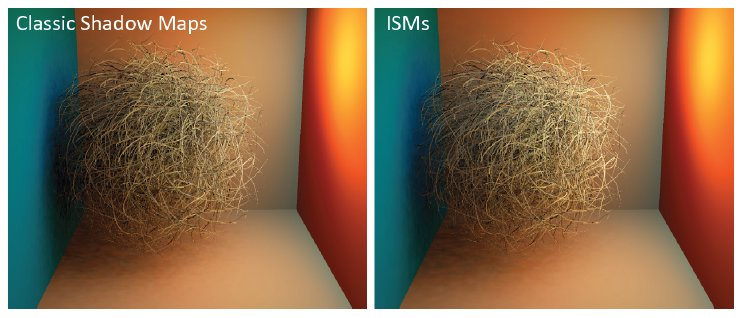
\includegraphics[width=1.0\textwidth]{ISMcompare.jpg}
  \caption{Comparison of normal shadow maps and ISM's.}
	\label{fig:ISMcompare}
\end{figure}

\paragraph{}
\underline{Screen Space Algorithms}: Additional VPL variants include \textit{Hierarchical Image-Space Radiosity for Interactive Global Illumination} by Nichols, Shopf, and Wyman (2009) where instant radiosity is combined with multiresolution techniques by Nichols and Wyman (2009).  This is done by accumulating indirect illumination at a variety of different resolutions in image space depending upon singularities.  When no singularities are nearby, a lower resolution can be used whereas when there are singularities, a higher resolution should be used to avoid artifacts.  Similar to many of the previous methods mentioned, this techniques ignores visibility for indirect light.

\paragraph{}
Lastly, VPL approaches can introduce bias.  When a VPL is close to a surface, it will introduce a singularity that appears as a high intensity peak in the image.  Most techniques solve this by clamping a VPL's contribution to a surface if it is nearby, however, this removes energy from the system and therefore introduces a bias.  This bias results in darkening of the image near singularity areas such as wall boundaries and edges of objects.  In order to prevent this, screen-space bias compensation by Novák, Engelhardt, and Dachsbacher (2011) was introduced as a post-processing step to recover the clamped energy.  This step involves applying a residual operator to the direct illumination and clamped indirect illumination as computed through the use of the rendering equation (equation \ref{eqn:render}) and a new residual operator.

\subsection{Spherical Harmonics and Lattice-Based Methods}
\paragraph{}
Spherical harmonics are the angular portion of a set of solutions to Laplace's equation represented in a system of spherical coordinates.  Nijasure, Pattanaik, and Goel (2005) used them as a way to represent the incident light at each sample point on a regular grid comprised of both direct and indirect light that arrives from all surface points visible to that sample point in a compact way.  This compact representation is comprised of a small number of coefficients that are computed through the use of a spherical harmonics transformation.  The incident radiance is approximated through the use of a cube map at each grid point, stored as spherical harmonics coefficients, and then the indirect illumination is calculated by interpolating the radiance at the nearest grid points.  This techniques allows for indirect occlusion through the use of shadow cube maps, but is expensive for complicated dynamic scenes.  Papaioannou (2011) combined the grid-based radiance caching of Nijasure et al. (2005) and the use of spherical harmonics along with the reflective shadow maps discussed earlier.  Instead of using cube maps to sample the visibility, this technique sampled the RSM to increase performance.  Kaplanyan and Dachsbacher (2010) used a volume-based method with lattices and spherical harmonics to represent the spatial and angular distribution of light in the scene where VPL's from a RSM are inserted into a volume texture.  This light propagation volume allows for iterative propagation of energy among voxels as well as accounting for fuzzy occlusion by storing depth information and RSM's in a separate occlusion volume to compute indirect shadows that are limited to surfaces larger than the grid size.  These light propagation volumes allow for the use of many more VPL's than other methods due to not calculating the contribution of each of the VPL's individually.  The occlusion calculations are also view-dependent which leads to problems such as popping artifacts.
\chapter{IMPLEMENTATION}

\section{IMPLEMENTATION GOALS} \label{sec:impgoals}

The goal of this implementation is to propose a real-time rendering technique that will render global illumination on the GPU through the use of OpenGL and GLSL.  We will use the idea of virtual point lights from \textit{Instant Radiosity} \cite{Keller1997} to render the indirect illumination.  Shadow maps will be used as in the spirit of \cite{Williams1978} and \cite{Reeves1987} to render shadows for direct illumination.  The VPL's will be structured outward from a primary light source in a lattice.  These VPL's will be structured in specific distances and angles around the primary light source in hemispheres. The goal is to simulate multiple waves of VPL's flowing outward from the primary light source in order to simulate the light transport as wave-like in order to simulate indirect illumination using only the direct illumination of many VPL's while ignoring the bouncing of light among surfaces.  This way, we simulate light as a particle by using VPL's and as a wave in the way the VPL's will be organized.  This will allow the “wrapping” of light around objects in order to illuminate surfaces that may not be directly visible from the light source.  An additional goal of this implementation is to have the resulting technique be scalable.  The organization of the VPL's will allow us to use more or less VPL's depending on quality and performance desires.  Specific implementation details will follow in section \ref{sec:impdetails}.  Lastly, in support of this technique and its ignorance of calculating indirect illumination and instead use a direct illumination approximation of indirect illumination, we discuss the importance of scientifically correct rendering versus visually appealing rendering.

\section{SCIENTIFICALLY CORRECT VERSUS VISUALLY APPEALING}

All of the previous work mentioned in section \ref{sec:prevwork} used approximations when computing indirect illumination to varying degrees.  This is because as mentioned in section \ref{sec:render}, the rendering equation (equation \ref{eqn:render}) is calculated using a Neumann series and in order to get an exact calculation, an infinite number of iterations would need to be carried out to fully calculate the result.  These iterations account for the infinite number of indirect light bounces that take place.  Since this is unfeasible, approximations are made based off our demands for performance or realism.  For real-time applications, we must err on the side of performance, but since the presence of indirect light has been shown to be perceptually important we can't just simply ignore it either \cite{Stokes2004}.  Also, according to \cite{Stokes2004}, diffuse indirect illumination is perceptually the most important component to consider.  However, as the notion of “realism” is merely whether the rendering is visually pleasing to the human eye, major approximations can be made to increase performance provided the result is visually pleasing.  As such, we ignore the bouncing of light and try to approximate it with just cheap direct lighting that will be able to reach surfaces that otherwise only indirect light would reach in order to simulate the “feeling” of indirect light.  Proof of the idea that visually pleasing is sufficient is provided next.

In \textit{Perceptual Influence of Approximate Visibility in Indirect Illumination} \cite{Yu2009} it is proven that “accurate visibility is not required and that certain approximations may be introduced.”  When a person sees lighting rendered in a scene or in real-life, the most revealing or obvious lighting is the direct illumination.  When it is approximated or incorrect, it is apparent right away due to the high-frequency nature of direct lighting.  Indirect lighting, however is usually low-frequency and therefore has smooth graduations in changes of intensity.  This allows for more leeway for approximations and interpolations.  The most expensive calculation being visibility determination for indirect illumination.    To research the effects of this on the viewer's perception of the rendering, \cite{Yu2009} conducted a psychophysical study involving two different experiments.  The first experiment involved estimating the difference between the approximation rendering and the reference rendering based off of a number scale ranging from one to five corresponding to “not similar” and “extremely similar” respectively.  This experiment had 14 participants.  The second experiment involved ranking 10 approximated renderings and 1 reference rendering in order of least realistic to most realistic.  This experiment had 18 participants.  Over half of the participants in both experiments were computer  scientists with a background in imaging.  The approximated renderings consisted of four different categories of indirect visibility.  These were imperfect visibility \cite{Ritschel2008}, ambient occlusion \cite{Zhukov1998}, directional ambient occlusion \cite{Sloan2007} \cite{Ritschel2009}, and no visibility ie. visibility for indirect illumination is completely neglected \cite{Dachsbacher2005} and \cite{Dachsbacher2006}.  All the renderings were prerendered 5-second video sequences and consisted of four different test scenes.

The results showed that the imperfect visibility approximations were very much similar or moderately similar to the reference video in all scenes.  The ambient occlusion approximations were also very much similar or moderately similar to the reference video in most scenes.  Directional ambient occlusion was considered very much similar or moderately similar to the reference video in most scenes.  Lastly, the no visibility approximations were considered moderately similar to the reference video.  Also, there was found to be a connection between the amount of indirect illumination and the perceived similarity to the reference.  In terms of the perceived realism of the renderings, the reference video as well as the imperfect visibility, ambient occlusion, and directional ambient occlusion approximations were all considered equally realistic leaving just the no visibility approximations as less realistic than the rest.  Overall, the imperfect visibility approximations as in \cite{Ritschel2008} were considered the most realistic of the approximations.

This study shows that visibility approximations can be made when rendering indirect illumination while remaining perceptually similar or as realistic as a reference rendering.  This provides validity to the approximations already done as well as support further approximations to come.  Having the imperfect visibility methods declared as the most realistic leads to the assumption that randomly corrupted visibility is more pleasing than incorrect visibility.  Lastly, it is shown that although all the approximations had noticeable differences in the renderings, many of them were still thought of as being realistic.

\section{IMPLEMENTATION DETAILS} \label{sec:impdetails}

As stated in section \ref{sec:impgoals}, the goal of this implementation is to propose a real-time rendering technique that will render global illumination on the GPU through the use of OpenGL and GLSL.  The primary focus is to render indirect illumination with the findings on scientifically accurate versus perceptually pleasing in mind.  As such, we will ignore the indirect bouncing of light (the infinite series portion of the rendering equation), but try to simulate it using the VPL technique as introduced in \cite{Keller1997}.  We will accomplish this simulation through the method of VPL placement and handling.  The VPL's will be structured in hemispheres around the primary light source.  The default original implementation will include VPL's at every $5$ degrees around the y-axis of the light source resulting in 360 degrees / 5 degrees per ray = 72 rays of VPL's forming a circle around the light source. See figure \ref{fig:3.1}.

\begin{figure}[h!]
  \centering
    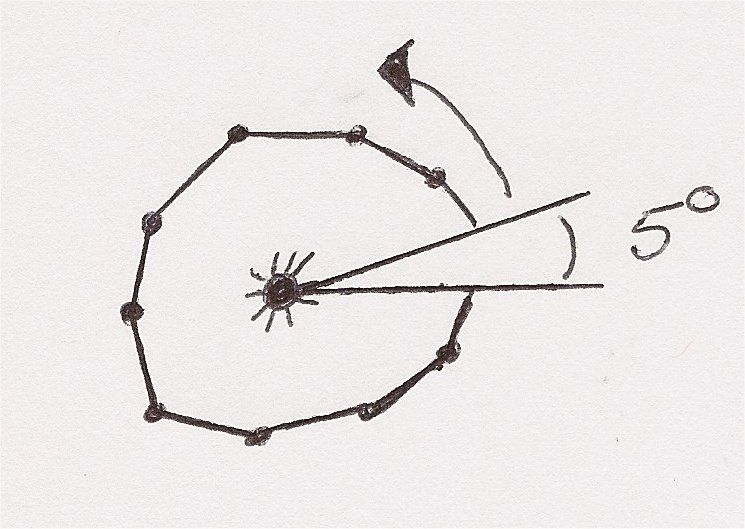
\includegraphics[width=0.5\textwidth]{Figure31.jpg}
  \caption{The light source is facing the reader (ie. direction/normal pointing out of the paper. Angles not drawn to scale.}
	\label{fig:3.1}
\end{figure}


Next, the VPL's will be structured at every 5 degrees around the z-axis of the light source resulting in 90degrees/5degrees per ray = 18 rays of VPL's for every one of the 72 rays around the z-axis.  This totals in 1296 rays plus the vertical ray along the z-axis resulting in 1297 rays to form a hemisphere around the light. See figures \ref{fig:3.2} and \ref{fig:3.3}.

\begin{figure}[h!]
  \centering
    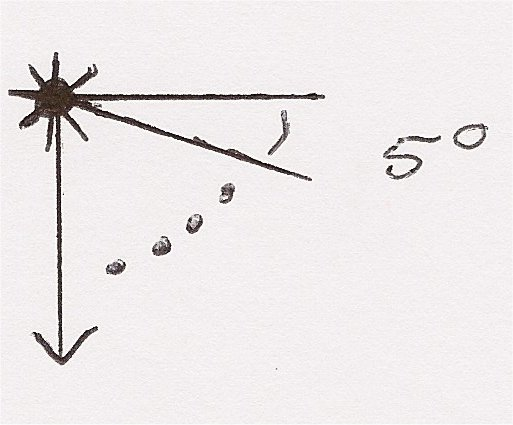
\includegraphics[width=0.5\textwidth]{Figure32.jpg}
  \caption{The light source is facing downwards. The arrow going down signifies the vertical ray added to the total of 1296 VPL's. Angles not drawn to scale.}
	\label{fig:3.2}
\end{figure}


\begin{figure}[h!]
  \centering
    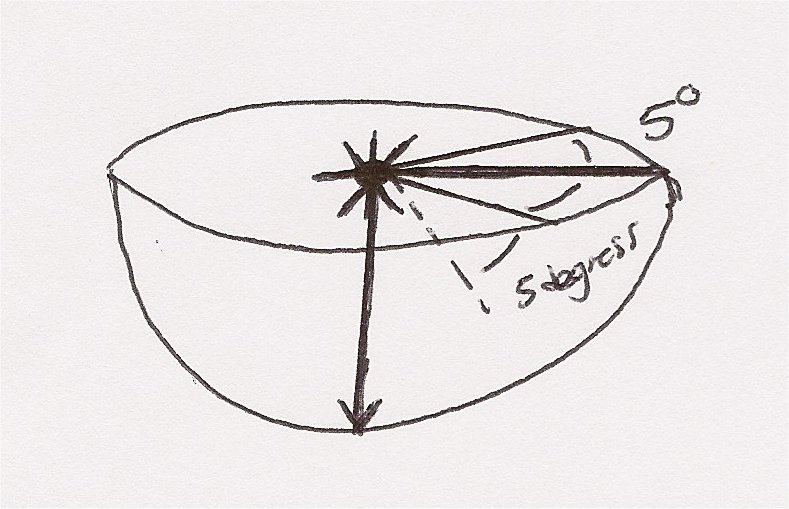
\includegraphics[width=0.5\textwidth]{Figure33.jpg}
  \caption{Figures \ref{fig:3.1} and \ref{fig:3.2} together form a hemisphere. The arrow signifies the primary light source's direction and is the additional vertical ray added to the total of 1296 VPL's.}
	\label{fig:3.3}
\end{figure}

Next, we will have multiple VPL's on each of these rays.  This implementation will have 5 VPL's per ray.  This results in having 5 stacked hemispheres of increasing radii and a total of 6485 VPL's. See figure \ref{fig:3.4}.

\begin{figure}[h!]
  \centering
    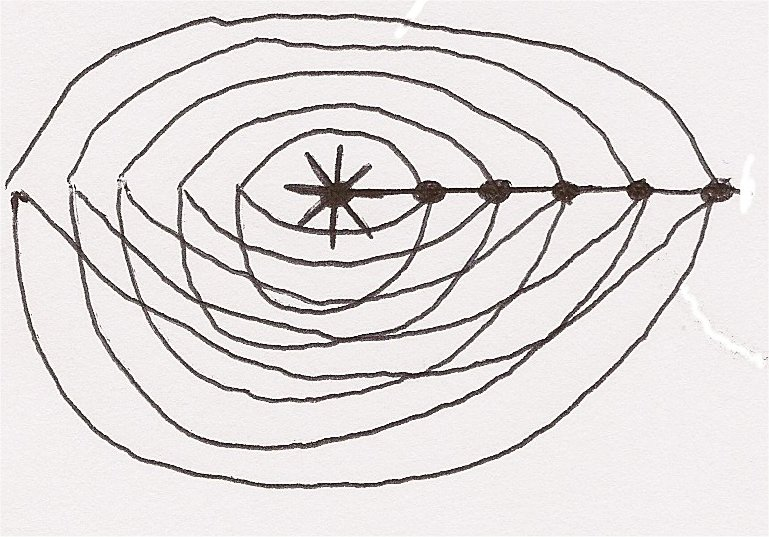
\includegraphics[width=0.5\textwidth]{Figure34.jpg}
  \caption{5 stacked hemispheres formed by the VPL's around the primary light source. Distances between hemispheres are not drawn to scale.}
	\label{fig:3.4}
\end{figure}

The distance from the primary light to each of the VPL's on each ray will be calculated based off of the depth of the scene.  The distance between VPL's on each ray will be logarithmic as shown below and the attenuation will be exponential.  See figure \ref{fig:3.5}.

\begin{figure}[h!]
  \centering
    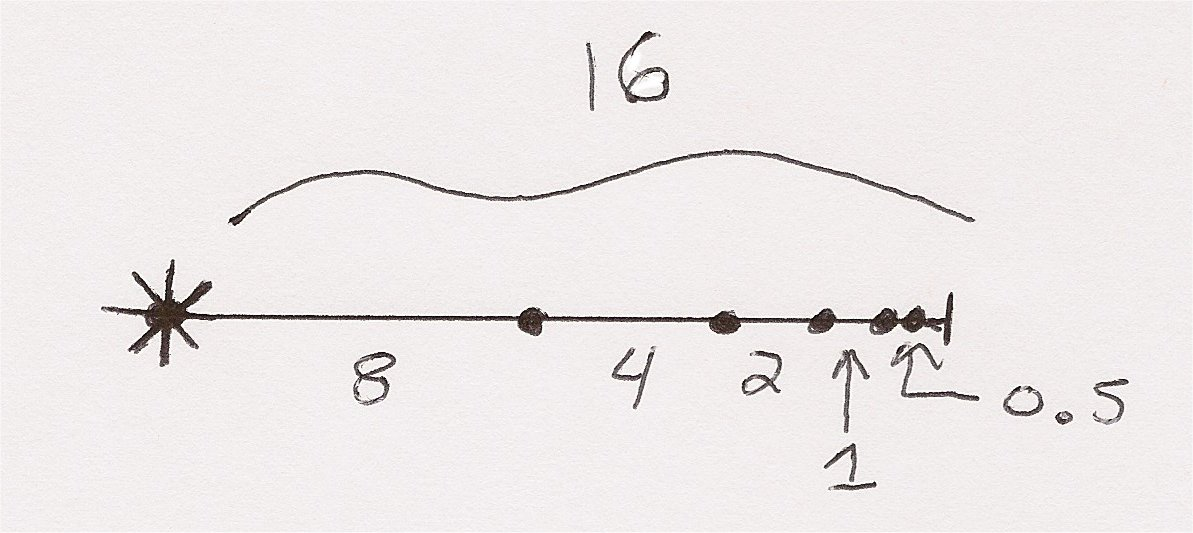
\includegraphics[width=0.5\textwidth]{Figure35.jpg}
  \caption{Showing the logarithmic structure of the VPL's.  Attenuation levels would be 5\%, 10\%, 20\%, 40\%, and 80\% from the left to right.}
	\label{fig:3.5}
\end{figure}

The goal of this structure is to simulate multiple waves of VPL's flowing outward from the primary light source in order to simulate the light transport as wave-like in order to simulate indirect illumination using only the direct illumination of these VPL's while ignoring the bouncing of light among surfaces.  An additional goal of this implementation is to have the resulting technique be scalable.  This organization of the VPL's will allow us to use more or less VPL's depending on quality and performance desires.  As such, we can increase or decrease the corresponding angles to reduce or increase the number of VPL's used as well as increase or decrease the number of hemisphere shells used.  Also, we can use stochastic sampling in order to turn off or on certain VPL's in order to introduce “noise” in the implementation as well as decrease the number of VPL's required.  As shown in the previous section, noise can be perceptually pleasing provided it is in smooth graduations.

The VPL's contributions will computed as shown in figure \ref{fig:3.6}.  The VPL's will act similar to directional lights in that the normal of the VPL will be used in computing the radiance that it provides.  The major difference, however, is that the VPL will be able to contribute radiance to surfaces that are slightly behind the VPL's normal.  Instead of doting the surface normal with the VPL normal and only allowing for contribution when the dot product is between 0 and 1, we will allow the dot product to be between -0.5 and 1.  This will mean that the VPL's viewable range is 240 degrees instead of 180 degrees.  This further depicts each VPL as wave-like.  The calculation to account for the expanded dot product range will be discussed along with the code explanations of chapter 4.  See figure \ref{fig:3.6}.

\begin{figure}[h!]
  \centering
    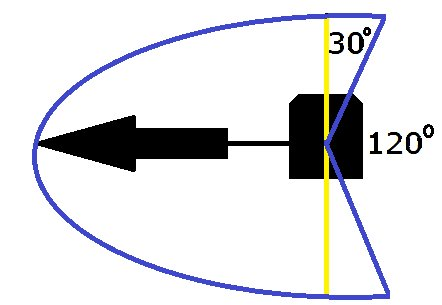
\includegraphics[width=0.5\textwidth]{Figure36.jpg}
  \caption{Showing the radiance contribution of a VPL on a surface point based off whether it is in front or behind the light.  The arrow signifies the VPL's direction/normal.}
	\label{fig:3.6}
\end{figure}

Occlusion will be handled with a shadow map as in \cite{Williams1978} and \cite{Reeves1987} to render shadows for the direct illumination based solely off of the primary light source.  This method is very cheap and provides sufficient shadows for the purposes of this implementation.  The indirect occlusion will be handled through the use of regular shadow maps on stochastically sampled VPL's.  This implementation will use 20 randomly chosen VPL's to derive indirect shadows.  The specific implementation details will be discussed in chapter 4 with code excerpts present.

\subsection{GPU AND CPU FUNCTIONS}

This implementation will be designed to use both the CPU and the GPU.  The CPU will handle all preliminary tasks such as setting up the window, initializing variables and the shaders, setting up the scene including position for the light source and objects, handling interactive actions including keyboard callbacks, initializing and filling textures, and initializing the VPL's position, direction, and attenuation.  The GPU will calculate shading and illumination based off vertices inputted along with the VPL texture and calculate shadows based off the provided shadow maps passed in from the CPU.

\subsection{OPENGL}

OpenGL or Open Graphics Library is a multi-platform API for graphics that will be used for this implementation.  The technique is being designed on a machine with OpenGL 4.2.0, however, OpenGL 2.1 and above will be supported.  Also, the technique will run on both Windows and Macintosh.

\subsection{GLSL}

GLSL or OpenGL Shading Language is a high-level C-syntax shading language to be used with OpenGL in order to give the developer control over what instructions are executed in the vertex and fragment shaders of the graphics pipeline.  In this implementation, all illumination and shading calculations are computed in the vertex and fragment shaders programmed manually through the use of GLSL.  The technique is being desgned on a machine with GLSL 4.20 support, but the shaders are written with GLSL 1.20 support.

\subsection{WORKING ENVIRONMENT}

The implementation is being designed and tested on the following hardware and software using the following libraries.  Any and all results such as rendered images and fps results will be gathered while running the method on the following.

\vspace{10 mm}

\textbf{HARDWARE}
\begin{itemize}
\item CPU: AMD Athlon 62 X2 Dual Core 5200+ 2.61Ghz
\item GPU: Nvidia GeForce GTX 465 (1GB memory)
\item Memory: 6.00GB
\end{itemize}

All other hardware specifications are irrelevant.

\vspace{10 mm}

\textbf{SOFTWARE}
\begin{itemize}
\item OS: Windows 7 64-Bit
\item Languages: C++, OpenGL 4.2.0 (2.1 tested/supported), OpenGL Shading Language 4.20 (written using version 1.20)
\item Developer Tools: Microsoft Visual Studio 2008
\end{itemize}

\vspace{10 mm}

\textbf{LIBRARIES}

\vspace{1 mm}

The following libraries are used in this implementation and provided in the repository.

\begin{itemize}
\item OpenGL Easy Extension Library (GLEE)
\item OpenGL Extension Wrangler Library (GLEW)
\item OpenGL Utility Toolkit (GLUT)
\end{itemize}


\chapter{SAMPLE CODE AND EXPLANATION}

\section{MAIN PROGRAM (C++ CODE)}
\paragraph{}
The main program is written in C++ using OpenGL and is run exclusively on the CPU.  It's responsibilities include setting up the window, initializing the shaders, and initializing and updating the textures and variables passed to the shaders.  After setting up the window, the first major step for the program is to generate the VPL's.  As discussed in section \ref{sec:impdetails} and in the associated figures, the default step up will include the use of 6485 VPL's.  The VPL's will be structured outward in hemispheres from the primary light source in the direction of the primary light source.  Assuming that the direction of the primary light source is pointing downward (negative y-axis), there will be a VPL at every 5 degrees around the y-axis for a total of 72 VPL's (360/5).  Then VPL's will be at every 5 degrees around the the z-axis resulting in 18 VPL's per 90 degree angle.  With this, our hemisphere is almost complete except for the VPL on the y-axis which is not included in the previous calculations. Therefore, we will have 1297 VPL's per hemisphere and 1297 outward rays.  Next, we will chose to have 5 stacked hemispheres flowing outward from the primary light source resulting in 6485 VPL's total.  

\paragraph{}
The locations of these VPL's will be calculated on start-up based on the location of the primary light source and the direction it is looking at.  The VPL's will only be updated whenever the primary light source is moved and at no other times reducing overhead.  The VPL's are calculated with an equation similar to below:

\begin{dmath}
vpl[x,y,z] = lightPosition[x,y,z] + normal[x,y,z]
	*(maxDistance - (maxDistance/2^i)) \label{eqn:vplPosition}
\end{dmath}

\paragraph{}
Equation \ref{eqn:vplPosition} calculates the position of the VPL by taking the position of the primary light source and moving in the direction of the primary light source by a particular distance and then rotating based on the angles required to fill the space in the hemisphere we are forming.  These angles are consolidated into the normal variable in equation \ref{eqn:vplPosition}.  The distance is calculated by using the maximum distance allowable (varies based off the dimensions of the scene) and the distances between each VPL on each outward ray is logarithmic which is achieved using $2^i$ where $i$ ranges from 1 to the number of hemispheres or 5 as is default with 1 being the innermost hemisphere and 5 being the outermost hemisphere.  Similarly, we get the VPL direction from rotating the primary light source direction to the direction of the corresponding VPL equal to the normal variable of equation \ref{eqn:vplPosition} as calculated by:

\begin{lstlisting}
normal[x,y,z] = primaryLightSourceNormal[x,y,z]
normal[x] = cos(angleZ*pi/180)*normal[x]-sin(angleZ*pi/180)*normal[y]
normal[y] = sin(angleZ*pi/180)*normal[x]+cos(angleZ*pi/180)*normal[y]
normal[x] = cos(angleY*pi/180)*normal[x]+sin(angleY*pi/180)*normal[z]
normal[z] =-sin(angleY*pi/180)*normal[x]+cos(angleY*pi/180)*normal[z]
\end{lstlisting}


Lastly, we get the attenuation from this exponential equation:

\begin{equation}
vplAttenuation = 0.05*pow(2.0,i)\label{eqn:vplAttenuation}
\end{equation}

\paragraph{}
Equation \ref{eqn:vplAttenuation} results in us getting the following attenuation levels for a VPL in each of the 5 hemispheres: $5\%, 10\%, 20\%, 40\%, 80\%$.  

\paragraph{}
Next, in order for the GPU to have access to the VPL data we have generated above, we store them somehow.  This is done by using 2 1D textures.  The VPL position data and normal data each receive their own texture.  The VPL position data texture is a RGB texture which stores float values of each of the xyz position values.  This is done in C++ with OpenGL by the following statement:

\begin{lstlisting}
glTexImage1D( GL_TEXTURE_1D, 0, GL_RGB, numLights, 0, GL_RGB, 
	GL_FLOAT, &vplDataPos[0]);
\end{lstlisting}

where numLights will be 6485 in this case and vplDataPos is the address for the VPL position data.  Similarly with the normal data we use a 1D texture but this time with RGBA since we will also store the attenuation in addition to the xyz normal values.

\begin{lstlisting}
glTexImage1D( GL_TEXTURE_1D, 0, GL_RGBA, numLights, 0, GL_RGBA, 
	GL_FLOAT, &vplDataNor[0]);
\end{lstlisting}

\paragraph{}
One problem arises in that the texture will clamp the values stored between 0 and 1.  This is a problem because our VPL data may be negative and will likely be larger than 1 (depending on the dimensions of our scene).  Therefore, prior to storing our data, we must encode our data such that all values will be between 0 and 1 and we can then knowingly decode the data once the texture is in the shaders so our original values are preserved.  This can be done by the following equation:

\begin{equation}
vpl[data] = (vpl[data]/(4*maxDistance))+0.5 \label{eqn:vplEncode}
\end{equation}

\paragraph{}
Equation \ref{eqn:vplEncode} normalizes the data to be between -0.5 and 0.5 and then adds 0.5 to it to reach the required 0 to 1 range.  The normalization is primarily important to the VPL position data since the VPL normals are already between -1 and 1 and the attenuation is already between 0 and 1. Then once in the shader we can decode the data with the following:

\begin{equation}
vpl[data] = (vpl[data]-0.5)*maxDistance*4.0; \label{eqn:vplDecode}
\end{equation}

Once again, the above steps will only be done at initialization and whenever the primary light source is moved.

\paragraph{}
The next step is to generate our shadow maps.  As discussed in section \ref{sec:prevwork}, shadow maps are generated by viewing the scene from the perspective of the light source in question rather than from our camera.  Then we calculate the distance to the first surface in each pixel to find the depths of the scene.  Using this depth, we can compare the value with the depth of other surfaces and determine whether a point lies in shadow.  In the first technique, we use 21 shadow maps. One for the primary light source for direct shadows and 20 for the randomly chosen VPL's for the indirect shadows.  For the second technique, we use 6 shadow maps with 1 being used for direct shadows and the other 5 for indirect shadows.  The 5 VPL's chosen lie in the innermost hemisphere equal distant apart to get maximum coverage.  In order to store these shadow maps, we use a single 2D texture array which consists of either 6 or 21 layers.  This is done in OpenGL by using the following line of code:

\begin{lstlisting}
glTexImage3D(GL_TEXTURE_2D_ARRAY, 0, GL_DEPTH_COMPONENT32, SMWidth, 
SMHeight, numShadowMaps, 0, GL_DEPTH_COMPONENT, GL_FLOAT, NULL);
\end{lstlisting}

\paragraph{}
The above line of code uses the depth component since we are only interested in the depth value at each pixel and nothing else with shadow maps.  Next, we need the width and height of the shadow map and we declare that we will be storing floats.  The width and height of the shadow maps should be a ratio of the screen size.  Ideally, it should be a multiple larger.  In our case, we will have the shadow maps be three times larger than the screen size.  We want it to be larger in order to minimize any jaggies that would be clearly visible should the shadow maps be the same size or even smaller than the screen size.  We do have limitations on how large we want our shadow maps to be because of the amount of memory available on the GPU to store them.  Memory considerations and analysis will be discusses in chapter 5.  

\paragraph{}
Next, in order to capture the depth values of the scene we use OpenGL's frame buffer capabilities.  We render the scene either 6 or 21 times from the perspective of each light in question to generate the shadow maps and then use these to determine which points lie in shadow from each light's perspective for the final rendering which is the only rendering that the user sees.  While generating the shadow maps we are using the fixed function pipeline to perform the rendering from each perspective meaning that it is rendered entirely on the CPU using no modified shaders.  Each time we render the scene, we attach the frame buffer to our shadow map texture using the following:

\begin{lstlisting}
glFramebufferTextureLayer(GL_FRAMEBUFFER, GL_DEPTH_ATTACHMENT, 
	shadowMapTexture, 0, i);
\end{lstlisting}

where $i$ corresponds to which layer of the texture to attach it.  Next, in order for this shadow map to be useful we need a way to transform any given vertex to a coordinate in the shadow map.  We do this by storing the associated modelview and projection matrices used to render the scene each time in a uniform matrix variable that is passed over to the shaders on the GPU.  This way we will be able to take any vertex, transform it using our transformation matrix and find the correct coordinate in the shadow map to compare it's depth.  This can be done in OpenGL by:

\begin{lstlisting}
glUniformMatrix4fv(lightMatrix, numShadowMaps, GL_FALSE, 
	(GLfloat*)textureMatrix);
\end{lstlisting}

where lightMatrix corresponds to a OpenGL variable that stores the location of the matrix for the shaders, GL\_FALSE tells OpenGL to not transpose the matrix, and textureMatrix is where we are storing our modelview and projection matrices for each shadow map.  These shadow maps will be generated at initialization and for every frame where either an object or the primary light source is moved.

\paragraph{}
Next, the main thing left for the main program to perform is to render the final scene with the assistance of the shaders on the GPU, which will be discussed in the following sections.

\section{VERTEX SHADER CODE}
\paragraph{}
The vertex shader is run exclusively on the GPU and is programmed using GLSL or OpenGL Shading Language, which is very similar to C.  The vertex shader is ran for each individual vertex from our scene.  The primary tasks performed in the vertex shader for our program is transforming the input vertices, reading some of the textures and all of the uniform variables passed in from the CPU, calculating the per-vertex variables for direct lighting, calculating the VPL color contributions to indirect illumination, and calculating the corresponding shadow map coordinates.

\paragraph{}
Transforming each input vertex is an easy one-line statement:

\begin{equation}
gl\_Position = gl\_ModelViewProjectionMatrix * gl\_Vertex;
\end{equation}

Each of the above variables used in the line above are preallocated variables used in GLSL.

\paragraph{}
Next, we calculate the per-vertex variables for the direct lighting.  For our diffuse shading, we need the light direction which can be calculated using the following line:

\begin{equation}
lightDir = vec3(masterLightPosition) - gl\_Vertex.xyz;
\end{equation}

For the specular lighting used in our direct illumination, we need the direction of the light reflected as well as the viewing direction of our camera.

\begin{equation}
lightDirRef = reflect(-lightDir, gl\_Normal);
\end{equation}

\begin{equation}
camDir = vec3(cameraPosition) - gl\_Vertex.xyz;
\end{equation}

The reflect function is a built-in function that is part of the GLSL language.  

\paragraph{}
The next task is to calculate the VPL indirect lighting contributions.  For all 6485 VPL's, we first access our VPL data from our 2 textures using the following lines of code:

\begin{lstlisting}
vec3 vplPosition = texture1D(vplPosTex,texCoord).rgb;
vec3 vplNormal = texture1D(vplNorTex,texCoord).rgb;
float vplAttenuation = texture1D(vplNorTex,texCoord).a;
\end{lstlisting}

where vplPosTex and vplNorTex are our vpl position and normal/attenuation textures and texCoord is the location in that texture we need to access.  We have to calculate texCoord by using the line:

\begin{lstlisting}
float texCoord = (float(i)/numLights);
\end{lstlisting}

where i ranges from 1 to 6485 and numLights is 6485.  Once we have our data, we must decode as discussed earlier using equation \ref{eqn:vplDecode}.  

\paragraph{}
Now that we have our original VPL data, we must calculate the vector from our vertex to each VPL similar to lightDir above.  Next, we calculate the diffuse terms of the object reflection and of the directional light.  This is done by taking the dot product between the normal of the vertex and the vector from the vertex to the VPL and then taking the dot product between the normal of the VPL and the vector from the light to the vertex.  All of these vectors must be normalized prior to these calculations.

\paragraph{}
Next, as discussed in section \ref{sec:impdetails} and shown in figure \ref{fig:3.6}, we will widen the viewable angle of the VPL from 180 degrees to 240 degrees.  We do this by taking our diffuse term from directional light and normalize it to allow for a wider contributing angle by the following lines of code:

\begin{equation}
DiffuseTermLight = (DiffuseTermLight + 0.5)/1.5;
\end{equation}

\begin{equation}
DiffuseTermLight = clamp(DiffuseTermLight, 0.0, 1.0);
\end{equation}

This allows the dot product result to contribute to the color by mapping the range $[-0.5, 1.0]$ to the range $[0.0, 1.0]$ thus widening our VPL viewable contributions from 180 degrees to 240 degrees.

\paragraph{}
We then calculate the specular contributions of each VPL using the reflection ray from the normal of the vertex and the vector from the light to the vertex which is dotted with the view direction of the camera.

\paragraph{}
Lastly, we accumulate all of the VPL contributions to the color of that vertex by the following line:

\begin{dmath}
indirect\_color += gl\_Color*DiffuseTermObj*DiffuseTermLight
	*(1-vplAttenuation)+SpecularTerm;
\end{dmath}

where gl\_Color is the color of the input vertex.  We then divide this by the number of VPL's to get our final indirect color for that vertex.

\paragraph{}
Lastly, the vertex shader must compute the corresponding coordinate for the vertex in each of the shadow maps.  This is done by multiplying our vertex by the input modelview and projection matrices for each of the rendered views corresponding to each of our shadow maps.

\paragraph{}
The vertex shader then passes control on to the fragment shader.  It also must pass variables calculated over by using varying variables.  These variables include: light direction, light direction reflected ray, camera direction, and vertex normal for direct lighting, as well as our indirect color contributions per-vertex and the corresponding coordinates for the vertex in each of our shadow maps.

\section{FRAGMENT SHADER CODE}\label{sec:fragShader}
\paragraph{}
The fragment shader is similar to the vertex shader in operation except that it performs operations on fragments of our primitives rather than vertices.  The fragment shader will perform these operations using the varying variables passed in from the vertex shader as well as our 2D texture array shadow map.

\paragraph{}
The first task the fragment shader has is to calculate whether our fragment is in shadow.  For the first technique, we do this with the line:

\begin{lstlisting}
float shadow = shadow2DArray(ShadowMap, 
	vec4(ShadowCoord.xy / ShadowCoord.w, i, 
	ShadowCoord.z / ShadowCoord.w)).r;
\end{lstlisting}

where we take our shadow map and index using our coordinates calculated in the vertex shader which is then divided by the 4th component of the vector known as perspective divide.  This is necessary in order to index into our shadow map, because our texture is in the range $[0.0, 1.0]$ and our coordinates are not.  The i corresponds to the layer of the shadow map to index into.  Our direct shadow map then will have $i=0$ and our indirect shadow maps will range from 1 to 20.  We do this for all 21 shadow maps.  From this we get a float value for our direct shadows that will range from 0 to 1.  We will also get a float value for our indirect shadows that after we divide by 20 to normalize the shadowing will also range from 0 to 1.  This float value corresponds to the percentage of shadowing with 0 meaning no lighting whatsoever and 1 meaning no shadowing whatsoever for that particular fragment.  This resulting value from the direct shadow map is then multiplied with our direct lighting and the resulting normalized value from our indirect shadow maps is multiplied with our indirect lighting.

\paragraph{}
For the second technique, we use the same line above for our direct shadows ($i=0$) and for each of our 5 indirect shadow maps.  However, the only difference in this technique is that we then integrate between each of these 5 indirect shadow maps in order to render additional shadows.  This is done by creating a vector that goes from the coordinate of one shadow map to the other.  We then divide this vector by the number of between steps we want to take.  We will show results based off using 2, 4, 6, and 10 as the number of steps. Then we step across this vector using the chosen number of steps to calculate the in-between coordinate which then contributes an additional indirect shadow.  We use the above line along with our in-between coordinate as the ShadowCoord to get our float value.  For the value of i in the above equation, we round to the closest shadow map. So for example, if we are integrating between $i=1$ and $i=2$ and using 10 steps, the first 5 coordinates will be using $i=1$ and the last 5 coordinates will be using $i=2$.  

\paragraph{}
We then do this for all combinations of the indirect shadow maps.  By combinations, we mean the act of selecting a subset of k distinct elements in a set S which can be calculated by using the binomial coefficient (equation \ref{eqn:binomial}).

\begin{equation}
\left(
    \begin{array}{c}
      n \\
      k
    \end{array}
  \right) = \frac{n!}{k!(n-k)!} \label{eqn:binomial}
\end{equation}

Here n is the number of elements in set S which in our case will be 5 for the number of indirect shadow maps.  Then we have $k=2$ because we want to create a vector between 2 indirect shadow maps.  This leads to equation \ref{eqn:binomialSolved}.

\begin{equation}
\left(
    \begin{array}{c}
      5 \\
      2
    \end{array}
  \right) = \frac{120}{2*6} = 10\label{eqn:binomialSolved}
\end{equation}

Therefore, we create 10 vectors between our 5 indirect shadow maps (1-2, 1-3, 1-4, 1-5, 2-3, 2-4, 2-5, 3-4, 3-5, 4-5).  Then we add all of the resulting shadowing values and divide by the number of shadows to normalize, which depends on the number of steps we take:

\begin{equation}
numShadows = (numSteps+2)*10\label{eqn:numIndShadows}
\end{equation}

where 10 comes from equation \ref{eqn:binomialSolved}.  So for 2 steps, we get 40 indirect shadows and for 10 steps we get 120 indirect shadows.  Most of these shadows are not using accurate visibility, but the act of integrating between shadow maps that are using accurate visibility provide us with overall smoother shadows while also using less shadow maps and therefore less GPU memory.

\paragraph{}
Next, we finish our direct lighting calculations by calculating the diffuse and specular terms similar to our indirect lighting in the vertex shader and add them for our direct lighting contributions.

Lastly, we set the color of the fragment using the line:

\begin{equation}
gl\_FragColor = (direct\_color*shadow) + (indirect\_color*INDshadow); \label{eqn:fragColor}
\end{equation}

where shadow and INDshadow are the float values we calculated above from our shadow maps, direct color is our direct lighting we have just calculated and indirect color is the VPL contributions we calculated in our vertex shader.  After performing equation \ref{eqn:fragColor}, we have our scene rendered with approximated global illumination by using our VPL's.

\chapter{RESULTS}

\section{RESULTS}
In order to give a detailed display of the flexibility of this method, we wanted to show the results of the method after changing many of the parameters.  These include varying the resolution of the screen, angle of between VPL rays, number of VPL's per ray, and number of indirect shadow maps used. Modifying these parameters will have an impact on performance or number of frames rendered per second as well as quality.  Therefore, section \ref{sec:fps} will detail the performance impact of varying the parameters based off the change in the number of frames per second rendered and section \ref{sec:quality} will detail the impact of varying the parameters on the quality of the images rendered by calculating the percentage difference per pixel against the default parameter set-up.  As a reminder, the default method which is featured first on each table uses a resolution size of 1280 by 720, an angle of 5 degrees between VPL rays, 5 VPL's per ray, and 20 indirect shadow maps.

\subsection{IMPACT OF PARAMETER CHOICES ON FPS} \label{sec:fps}
The results will given in frames per second (FPS).  Table \ref{table:5.1} will display the results of varying the angle between the VPL rays. Table \ref{table:5.2} will display the results of varying the number of VPL's used on each ray (the total number of hemispheres). Table \ref{table:5.3} will display the results of using varying the resolution used.  Lastly, \ref{table:5.4} will display the results of reducing the number of indirect shadow maps used.

\begin{table}[h!]
	\caption{Varying the Angle Between VPL Rays (Impact on FPS)}
	\begin{center}
	    \begin{tabular}{ | l | l | l | l | l | l |}
	    \hline
	    Resolution & Angle & VPL's Per Ray & Total \#VPL's & \#Indirect SM's & FPS\\ \hline
	    1280x720 & 5 & 5 & 6485 & 20 & 55\\ \hline
	    1280x720 & 10 & 5 & 1625 & 20 & 65\\ \hline
	    1280x720 & 30 & 5 & 185 & 20 & 84\\ \hline
	    1280x720 & 45 & 5 & 85 & 20 & 95\\ \hline
	    1280x720 & 90 & 5 & 25 & 20 & 100\\ \hline
	    \end{tabular}
	\end{center}
	\label{table:5.1}
\end{table}

\begin{table}[h!]
	\caption{Varying the Number of VPL's Per Ray (Impact on FPS)}
	\begin{center}
	    \begin{tabular}{ | l | l | l | l | l | l |}
	    \hline
	    Resolution & Angle & VPL's Per Ray & Total \#VPL's & \#Indirect SM's & FPS\\ \hline
	    1280x720 & 5 & 5 & 6485 & 20 & 55\\ \hline
	    1280x720 & 5 & 4 & 5188 & 20 & 56\\ \hline
	    1280x720 & 5 & 3 & 3891 & 20 & 61\\ \hline
	    1280x720 & 5 & 2 & 2594 & 20 & 62\\ \hline
	    1280x720 & 5 & 1 & 1297 & 20 & 78\\ \hline
	    1280x720 & 5 & 6 & 7782 & 20 & 52\\ \hline
	    \end{tabular}
	\end{center}
	\label{table:5.2}
\end{table}

\begin{table}[h!]
	\caption{Varying the Resolution Size. (Impact on FPS)}
	\begin{center}
	    \begin{tabular}{ | l | l | l | l | l | l |}
	    \hline
	    Resolution & Angle & VPL's Per Ray & Total \#VPL's & \#Indirect SM's & FPS\\ \hline
	    1280x720 & 5 & 5 & 6485 & 20 & 55\\ \hline
	    1120x630 & 5 & 5 & 6485 & 20 & 82\\ \hline
	    960x540 & 5 & 5 & 6485 & 20 & 104\\ \hline
	    800x450 & 5 & 5 & 6485 & 20 & 119\\ \hline
	    640x360 & 5 & 5 & 6485 & 20 & 133\\ \hline
	    1440x810 & 5 & 5 & 6485 & 20 & 42\\ \hline
	    \end{tabular}
	\end{center}
	\label{table:5.3}
\end{table}

\begin{table}[h!]
	\caption{Varying the Number of Indirect Shadow Maps (Impact on FPS)}
	\begin{center}
	    \begin{tabular}{ | l | l | l | l | l | l |}
	    \hline
	    Resolution & Angle & VPL's Per Ray & Total \#VPL's & \#Indirect SM's & FPS\\ \hline
	    1280x720 & 5 & 5 & 6485 & 20 & 55\\ \hline
	    1280x720 & 5 & 5 & 6485 & 15 & 87\\ \hline
	    1280x720 & 5 & 5 & 6485 & 10 & 106\\ \hline
	    1280x720 & 5 & 5 & 6485 & 5 & 128\\ \hline
	    1280x720 & 5 & 5 & 6485 & 1 & 157\\ \hline
	    1280x720 & 5 & 5 & 6485 & 0 & 161\\ \hline
	    \end{tabular}
	\end{center}
	\label{table:5.4}
\end{table}

Tables \ref{table:5.1}, \ref{table:5.2}, \ref{table:5.3}, and \ref{table:5.4} show some important characteristics.  First, tables \ref{table:5.1} and \ref{table:5.2} shows the impact of the angle between rays and the number of VPL's per ray on the total number of VPL's used.  The equation to calculate the total number of VPL's based off the angle and the number of VPL's per ray used is:

\begin{equation}
numberVPLs = VPLsPerRay*((90/Angle)*(360/Angle)+1)
\label{eqn:calcVPLtotal}
\end{equation}

More interestingly, it shows that a large difference between the total number of VPL's used has a relatively small affect on the FPS recorded compared to other changes.  For example, reducing the number of VPL's used by a factor of 4 (from 6485 to 1625) increases FPS by only 10 whereas reducing the number of VPL's used by a factor of near 76 (from 6485 to 85) increases FPS by 40.

Table \ref{table:5.3} shows that decreasing the resolution of the screen has a relatively large impact on the FPS recorded.  To compare it against decreasing the number of VPL's used, in order to see a similar impact of reducing the resolution by 77\% or a factor of 1.3, we would have to reduce the number of VPL's by a factor of 35 (from 6485 to 185).

Similarly, table \ref{table:5.4} shows the number of indirect shadow maps having a relatively large impact on the performance.  As mentioned often in similar studies on indirect illumination, calculating indirect shadows is computationally expensive as supported in table \ref{table:5.4}.  To make a similar comparison as above, reducing the number of shadow maps used by 5, a factor of 1.33 or 75\%, has a similar impact as reducing the resolution by 77\% or a factor of 1.3 or reducing the number of VPL's by a factor of 35 (from 6485 to 185).  Also, table \ref{table:5.4} shows that for each indirect shadow map we add, we can expect a decrease in FPS by about 5.

In summary, when choosing parameters of the method to be run on slower machines, a combination of reducing the resolution and reducing the number of indirect shadow maps would result in the most efficient performance gain in regards to FPS increase.  Next, we will similarly analyze the impact of these parameter changes to the quality of the image in order to see what changes would result in the most efficient reductions while maintaining quality.

\subsection{IMPACT OF PARAMETER CHOICES ON QUALITY} \label{sec:quality}
Just as important as performance is the quality of the images rendered.  Therefore, this section will detail the quality impact of parameter choice using the default set-up as the reference image.  By detailing this information, it will reveal the ultimate flexibility of the method and whether we can use this method on slower machines with limited quality impact.  We will use the same parameter choices as the tables for section \ref{sec:fps}, but we will be interested in the percentage difference between the chosen parameters and the default parameters.  The percentage difference will be computed using a Python script which takes in two rendered images as input and compares them on a pixel by pixel basis.  This comparison is done as follows:


\begin{algorithm}[H]
 \SetAlgoLined
 similar = 0.0\;
 \For{each pixelComponent (R,B,G) in image 1}{
  \eIf{pixelComponent\_image1 $>=$ pixelComponent\_image2 }{
   similar += (pixelComponent\_image1 +1) / (pixelComponent\_image2 +1)\;
   }{
   similar += (pixelComponent\_image2 +1) / (pixelComponent\_image1 +1)\;
  }
 }
 similar = similar/numPixelComponents\;
 percentDifference = (1-similar)*100\;
 \caption{Compute Image Difference}
 \label{alg:difference}
\end{algorithm}

Algorithm \ref{alg:difference} adds 1 to the 2 pixel components in order to avoid division by 0.  This way our pixel components will range from 1 to 256.  For example, if image 1 had a value of 200 for the red component of pixel 1 and image 2 had a value of 100 for the red component of pixel 1, we would say that these two images were 50\% different.  We do this calculation for all 3 color components of every pixel in each image and average it out to find the total similarity or difference between the two images.

The purpose of doing such a calculation is simply due to the fact that quantifying the quality of an image or  the similarity with another image is rather subjective.  This way we can assign a value to the comparison which is more objective.  This way we can objectively order the images rendered using different parameters by similarity to the default parameter set-up and declare certain parameter changes as more efficient than others.  By efficient, we mean the parameter changes increase performance with limited quality reductions.  Tables \ref{table:5.5}, \ref{table:5.6}, \ref{table:5.7}, and \ref{table:5.8} show the calculated similarity percentages.  The higher percentage the image, the closer to the reference image it is with 100\% meaning that it is the same image.


\begin{table}[h!]
	\caption{Varying the Angle Between VPL Rays (Impact on Quality)}
	\begin{center}
	    \begin{tabular}{ | l | l | l | l | l | l |}
	    \hline
	    Resolution & Angle & VPL's Per Ray & Total \#VPL's & \#Indirect SM's & \% Similar\\ \hline
	    1280x720 & 5 & 5 & 6485 & 20 & 100\\ \hline
	    1280x720 & 10 & 5 & 1625 & 20 & 97.945\\ \hline
	    1280x720 & 30 & 5 & 185 & 20 & 97.956\\ \hline
	    1280x720 & 45 & 5 & 85 & 20 & 95.440\\ \hline
	    1280x720 & 90 & 5 & 25 & 20 & 92.676\\ \hline
	    \end{tabular}
	\end{center}
	\label{table:5.5}
\end{table}

\begin{table}[h!]
	\caption{Varying the Number of VPL's Per Ray (Impact on Quality)}
	\begin{center}
	    \begin{tabular}{ | l | l | l | l | l | l |}
	    \hline
	    Resolution & Angle & VPL's Per Ray & Total \#VPL's & \#Indirect SM's & \% Similar\\ \hline
	    1280x720 & 5 & 5 & 6485 & 20 & 100\\ \hline
	    1280x720 & 5 & 4 & 5188 & 20 & 92.973\\ \hline
	    1280x720 & 5 & 3 & 3891 & 20 & 93.458\\ \hline
	    1280x720 & 5 & 2 & 2594 & 20 & 90.318\\ \hline
	    1280x720 & 5 & 1 & 1297 & 20 & 91.591\\ \hline
	    1280x720 & 5 & 6 & 7782 & 20 & 96.509\\ \hline
	    \end{tabular}
	\end{center}
	\label{table:5.6}
\end{table}

\begin{table}[h!]
	\caption{Varying the Resolution Size. (Impact on Quality)}
	\begin{center}
	    \begin{tabular}{ | l | l | l | l | l | l |}
	    \hline
	    Resolution & Angle & VPL's Per Ray & Total \#VPL's & \#Indirect SM's & \% Similar\\ \hline
	    1280x720 & 5 & 5 & 6485 & 20 & 100\\ \hline
	    1120x630 & 5 & 5 & 6485 & 20 & 99.547\\ \hline
	    960x540 & 5 & 5 & 6485 & 20 & 99.541\\ \hline
	    800x450 & 5 & 5 & 6485 & 20 & 99.418\\ \hline
	    640x360 & 5 & 5 & 6485 & 20 & 99.483\\ \hline
	    1440x810 & 5 & 5 & 6485 & 20 & 99.741\\ \hline
	    \end{tabular}
	\end{center}
	\label{table:5.7}
\end{table}

\begin{table}[h!]
	\caption{Varying the Number of Indirect Shadow Maps (Impact on Quality)}
	\begin{center}
	    \begin{tabular}{ | l | l | l | l | l | l |}
	    \hline
	    Resolution & Angle & VPL's Per Ray & Total \#VPL's & \#Indirect SM's & \% Similar\\ \hline
	    1280x720 & 5 & 5 & 6485 & 20 & 100\\ \hline
	    1280x720 & 5 & 5 & 6485 & 15 & 99.475\\ \hline
	    1280x720 & 5 & 5 & 6485 & 10 & 98.853\\ \hline
	    1280x720 & 5 & 5 & 6485 & 5 & 93.611\\ \hline
	    1280x720 & 5 & 5 & 6485 & 1 & 90.897\\ \hline
	    1280x720 & 5 & 5 & 6485 & 0 & 98.563\\ \hline
	    \end{tabular}
	\end{center}
	\label{table:5.8}
\end{table}

Comparing tables \ref{table:5.5} and \ref{table:5.6} reveals that although the number of VPL's used when increasing our VPL ray angles drops more quickly than when we simply reduce the number of VPL per ray, the higher ray angle images (table \ref{table:5.5}) render more similar images to the reference than when we reduce the number of VPL per ray.  For example, when we use 185 VPL's with an angle of 30 degrees, we get an image that is 98\% similar to the reference, but when we use 1297 VPL's with 1 VPL per ray, we get an image that is only 91.6\% similar to the reference.  This leads us to believe that increasing the angle to reduce the number of VPL's leads to better quality images than reducing the number of VPL's per ray or hemispheres to reduce the number of VPL's.  Such an observation can helps us increase performance and maintain a level of similarity to the reference image.

When looking at table \ref{table:5.7}, we see high values of similarity to the reference, however, these can be misleading.  These values were calculated after rendering the image at the chosen resolution size and then stretching it to the reference image resolution size.  This brings into question the idea of global similarity and local similarity as well as notion of visually pleasing as discussed in section \ref{sec:study}.  Although these images are very similar to the reference in an overall pixel by pixel basis, there are some things that this number does not show us.  It requires looking at the stretched image to realize the effect this has on the image quality.  These images show worsening cases of 'jaggies' or artifacts near the edges of boundaries such as the edges of the boxes as the rendered image's resolution gets smaller.  So in the regard of being similar to the reference these reduced resolution images are, but when stretched they also show localized differences that can be distracting to the eye.  When comparing the reference to the stretched 640x360 images on a local scale such as on the edges of a box, we get a similarity of 97.4\% which is slightly less than the 99.5\%, however, a even more localized comparison such as a few pixels on either side of the boundary line would show even more difference.

Regardless of the calculations, a localized difference such as artifacts detract from the overall realism of the image which is not preferred.  A slight global difference, however, such as a slightly lighter or darker overall image would result in a large difference value but more similar overall to the human eye.  These facts need to be taken into consideration when choosing the method or parameters.  This idea will be covered more in section \ref{sec:alternatives}.

Table \ref{table:5.8} shows the impact of reducing the number of shadow maps used for indirect shadows.  An interesting note is that when using 10 shadow maps for indirect shadows and when completely ignoring indirect shadows we get near identical similarity measurements to our reference.  This reinforces the notion that indirect shadows are possibly an unnecessary computational burden that can be ignored especially on slower machines.  Recall table \ref{table:5.4} and the comparison of FPS between the two parameter choices.  When choosing to use 10 indirect shadow maps we get 106 FPS, however, when we ignore indirect shadows we get 161 FPS.  For nearly identical globally similarity values, we can gain 55 FPS by ignoring indirect shadows.  This is a major parameter choice to consider when wanting to increase performance.

It is worth noting that if an image is not 100\%, this does not mean that it is not a quality or accurate image rendering.  It purely means that the image is in some way different to our reference image.  For example, the last entry of table \ref{table:5.6} says that it is 96.5\% similar to our reference.  However, due to the fact that this rendering indeed uses more VPL's than our reference, this image could be perceived as more accurate or of higher quality than our reference.  This calculation does take into account the findings of section \ref{sec:study} which stated that there was found to be a connection between the amount of indirect illumination and the perceived similarity to the reference.  More on the idea of the amount of indirect illumination will be discussed in section \ref{sec:alternatives}.

\subsection{ALTERNATIVES} \label{sec:alternatives}
The aim of this section is to determine any additional sacrifices that could be made in order to improve performance.  As shown in table \ref{table:5.8} and discussed above, indirect shadowing is the most computationally expensive scene component that has the least influence of the overall scene.  This may lead one to consider whether or not ignoring indirect lighting could be possible.  However, as shown in table \ref{table:5.9}, we compared our default method with a direct lighting only method.  Using our similarity calculation, we see the lowest similarity of 84.4\%, but the highest performance with 681 FPS.  On a machine that is able to run any of the above parameter choices with at least 30 FPS, it is not necessary to sacrifice this much quality for performance, but for the slowest machines, this may be a necessary choice.

\begin{table}[h!]
	\caption{Alternative Reductions}
	\begin{center}
	    \begin{tabular}{ | l | l | l | l | l | l |}
	    \hline
	    Method & FPS & \% Similarilty to Default\\ \hline
	    Default Method & 55 & 100\\ \hline
	    Direct Lighting ONLY & 681 & 84.426\\ \hline
	    Indirect Lighting w/out indirect shadows & 161 & 98.563\\ \hline
	    Faked Indirect Lighting (1.1x) & 681 & 88.217\\ \hline
	    Faked Indirect Lighting (1.2x) & 681 & 90.675\\ \hline
	    Faked Indirect Lighting (1.3x) & 681 & 91.847\\ \hline
	    Faked Indirect Lighting (1.4x) & 681 & 91.393\\ \hline
	    Faked Indirect Lighting (1.5x) & 681 & 90.161\\ \hline
	    \end{tabular}
	\end{center}
	\label{table:5.9}
\end{table}

Also in table \ref{table:5.9}, we include our indirect lighting without indirect shadows method for comparison with it's respectable 161 FPS and 98.5\% similarity.  This was the best performing parameter choice from tables \ref{table:5.1} through \ref{table:5.4}.  Should a compromise between direct lighting only and indirect lighting with no indirect shadows be needed, we included a few alternative approaches in addition to the previous two in table \ref{table:5.9}.  These approaches attempt to fake indirect lighting while achieving the direct only performance.  This is done through the use of scaling the color and shadow contributions in the fragment shader.  As reminded above and discovered in section \ref{sec:study}, the amount of indirect light can contribute to the perceived realism of the scene.  As such, 5 different scaling approaches are included in table \ref{table:5.9} to compare against our reference image.  The multiplier in parenthesis in each table entry shows the amount of scaling done to the direct lighting of the scene.  For example, for the entry with a 1.1 multiplier this means that the final color is calculated as below:

\begin{equation}
color = (direct\_color*0.5*shadow)+(direct\_color*0.6)
\end{equation}

For the next entry the 0.6 would be 0.7 and so on.  This way the direct shadows are only half as dark as before and is not purely black and increase the overall brightness of the scene.  As seen in the table, this approach of faking indirect light leads to better similarity numbers than using just the direct lighting approach peaking at the multiplier of 1.3 with a value of 91.8\% in this particular case.  Therefore, should indirect lighting without indirect shadows approach be too much for a particular machine, a faked version of indirect lighting would be a respectable compromise.

\subsection{FINAL ANALYSIS} \label{sec:finalAnalysis}
Lastly, we will consolidate all of the previous data and tables in order to determine the most efficient reductions and the most influencing factors on the believability of the rendered scene.  The benefits of calculating similarities is that it leads to a way of quantifying quality in comparison to our reference image and thus rank parameter choices based off a combination of performance gains and limited quality impact.  It is important to note that changing the resolution size and stretching netted the best similarity results, but due to the introduction of artifacts, those parameter choices will not be included.  It is also important to note that should a smaller resolution size be applicable without the need to stretch to our larger default resolution, this should be the very first choice in increasing performance, because the artifacts are only introduced during the stretching process due to the method of likely naive sampling.

Table \ref{table:5.10} will use the similarity values calculated along with the FPS gain in order to rank the parameter choices.  This will be done using a simple equation:

\begin{equation}
rankValue = fpsGain / (1-calculatedSimilarity)
\end{equation}

\begin{table}[h!]
	\caption{Final Comparisons}
	\begin{center}
	    \begin{tabular}{ | l | l | l | l | l | l |}
	    \hline
	    Method & FPS & \% Similarilty to Default & Rank Value\\ \hline
	    Default Method & 55 & 100 & --\\ \hline
	    Faked Indirect Lighting (1.3x) & 681 & 91.847 & 76.7816\\ \hline
	    Indirect Lighting w/out indirect shadows & 161 & 98.563 & 73.7648\\ \hline
	    Indirect Lighting w/ 15 indirect shadows & 87 & 99.475 & 60.9524\\ \hline
	    Indirect Lighting w/ 10 indirect shadows & 106 & 98.853 & 44.4638\\ \hline
	    Direct Lighting ONLY & 681 & 84.426 & 40.1952\\ \hline
	    \hline
	    \hline
	    30 Degree Angle Between VPL Rays & 84 & 97.956 & 14.1879\\ \hline
	    \hline
	    \hline
	    Reduction down to 1 VPL Per Ray & 78 & 91.591 & 2.7352\\ \hline
	    \hline
	    \hline
	    Resolution Reduction 640x360 & 133 & 99.483 & 150.8704\\ \hline
	    \end{tabular}
	\end{center}
	\label{table:5.10}
\end{table}

Table \ref{table:5.10} tells us a few things:
\begin{itemize}
\item If a smaller resolution size can be used and not stretched, use it.
\item Indirect Shadows are nice, but is the next thing to be sacrificed if better performance is needed.
\item If we chose to reduce VPL's, do so by increasing the ray angles, not by reducing hemispheres.
\item We can experiment with multipliers and get decent faked indirect lighting if nothing else.
\end{itemize}

\section{IMAGES}
This section will be used to show images rendered in real-time from this method and the accompanying parameters chosen.


\begin{figure}[h!]
  \centering
    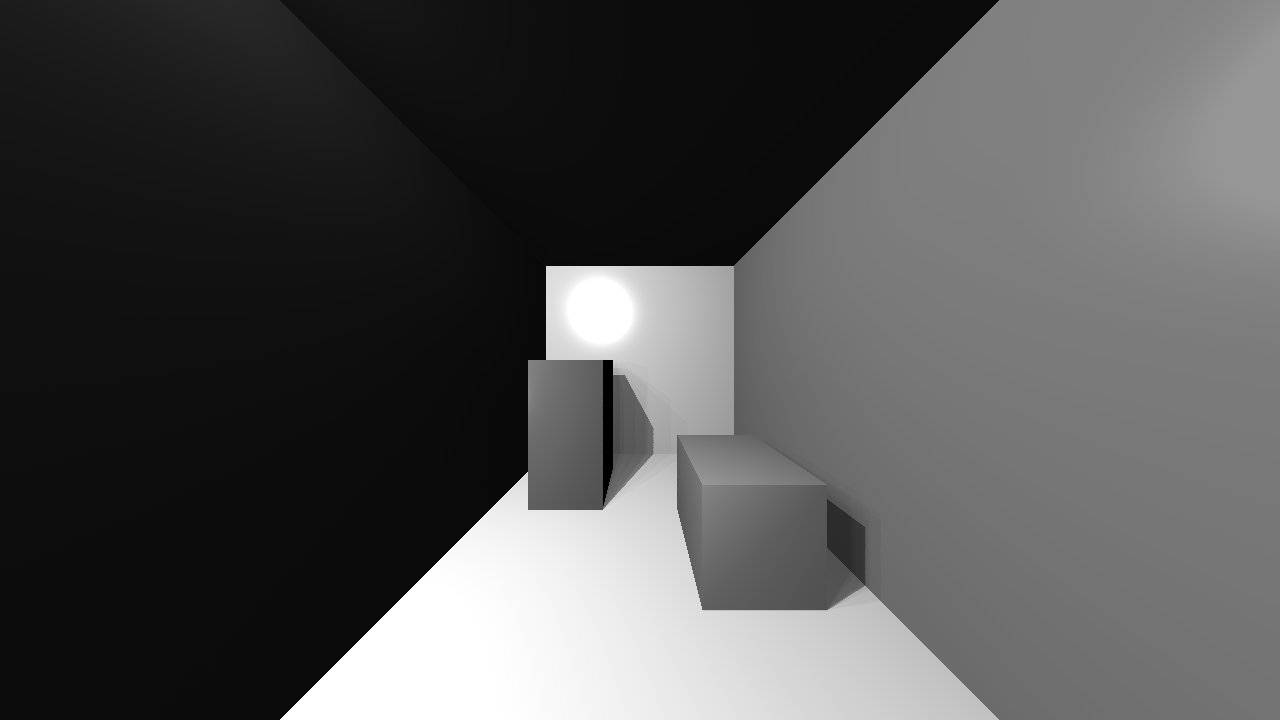
\includegraphics[width=1.0\textwidth]{sample1_gray.jpg}
  \caption{Light is at the near upper left corner of the scene. This image is used as the reference in the similarity calculations.}
	\label{fig:defaultimage}
\end{figure}


\begin{figure}
        \centering
        \begin{subfigure}[b]{0.5\textwidth}
                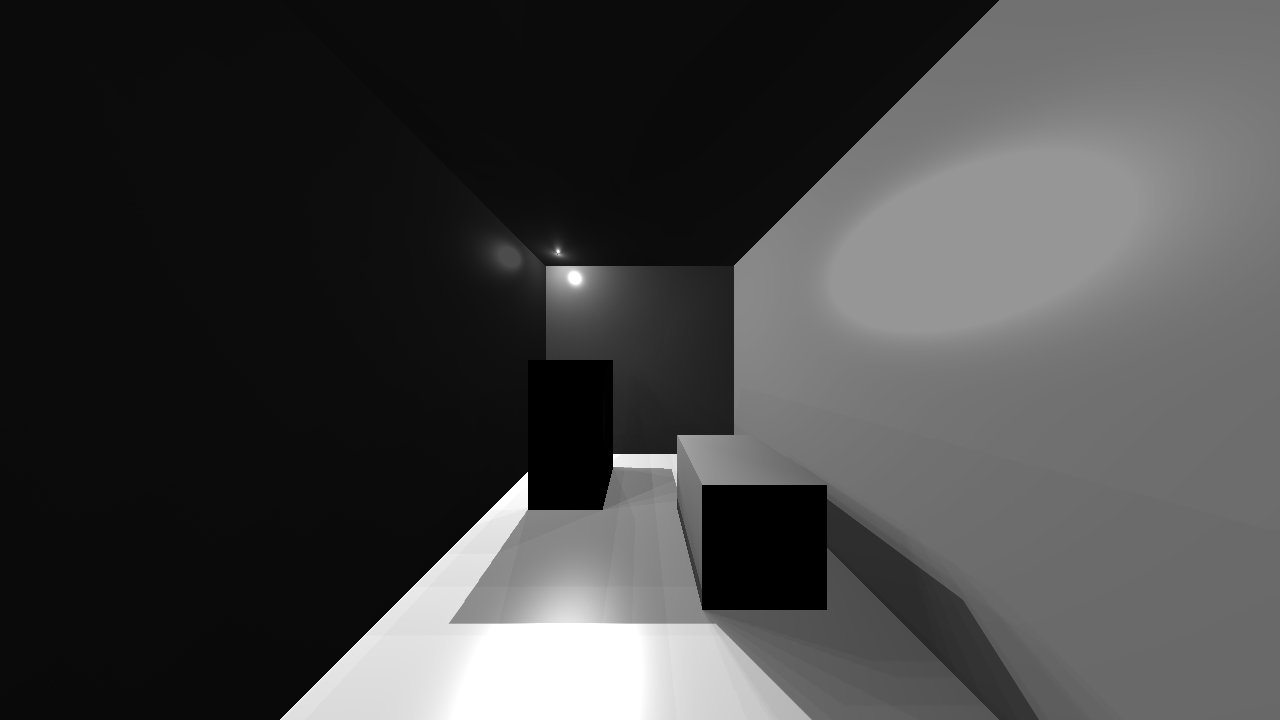
\includegraphics[width=\textwidth]{sample2_gray.jpg}
                \caption{Light is at the far upper left corner of the scene.}
                \label{fig:sample2}
        \end{subfigure}
        \begin{subfigure}[b]{0.5\textwidth}
                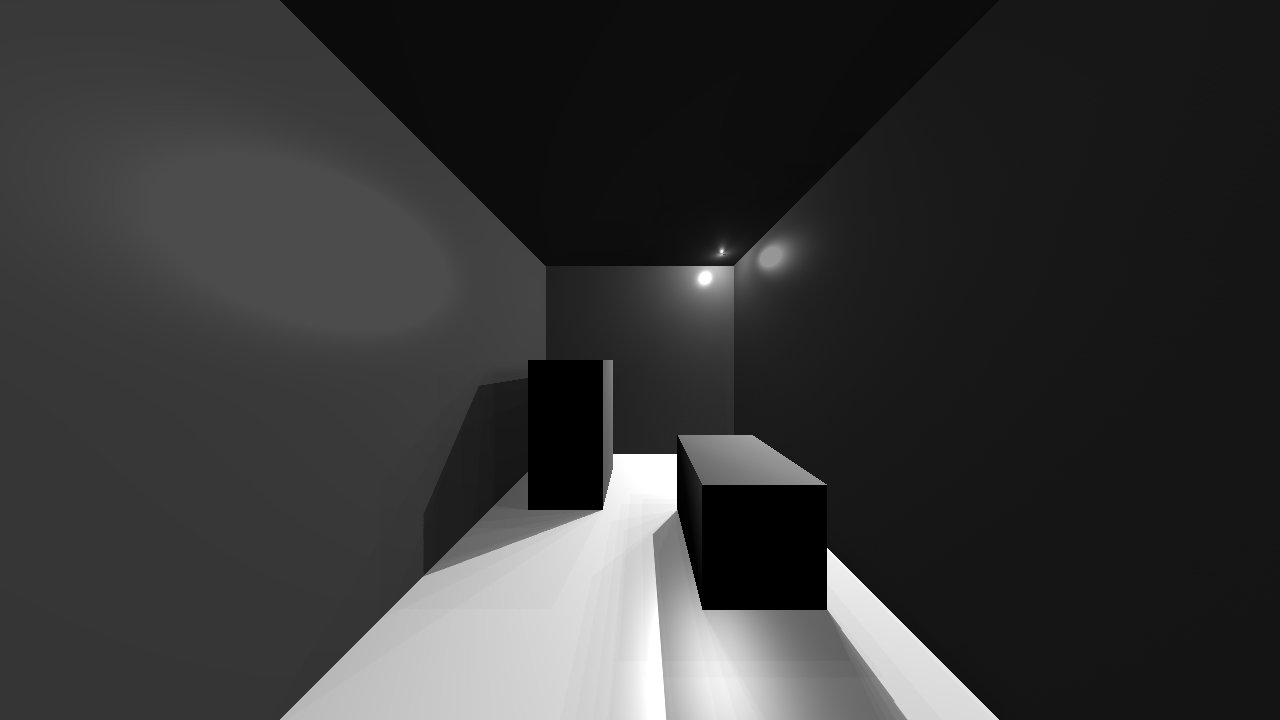
\includegraphics[width=\textwidth]{sample3_gray.jpg}
                \caption{Light is at the far upper right corner of the scene.}
                \label{fig:sample3}
        \end{subfigure}
        \begin{subfigure}[b]{0.5\textwidth}
                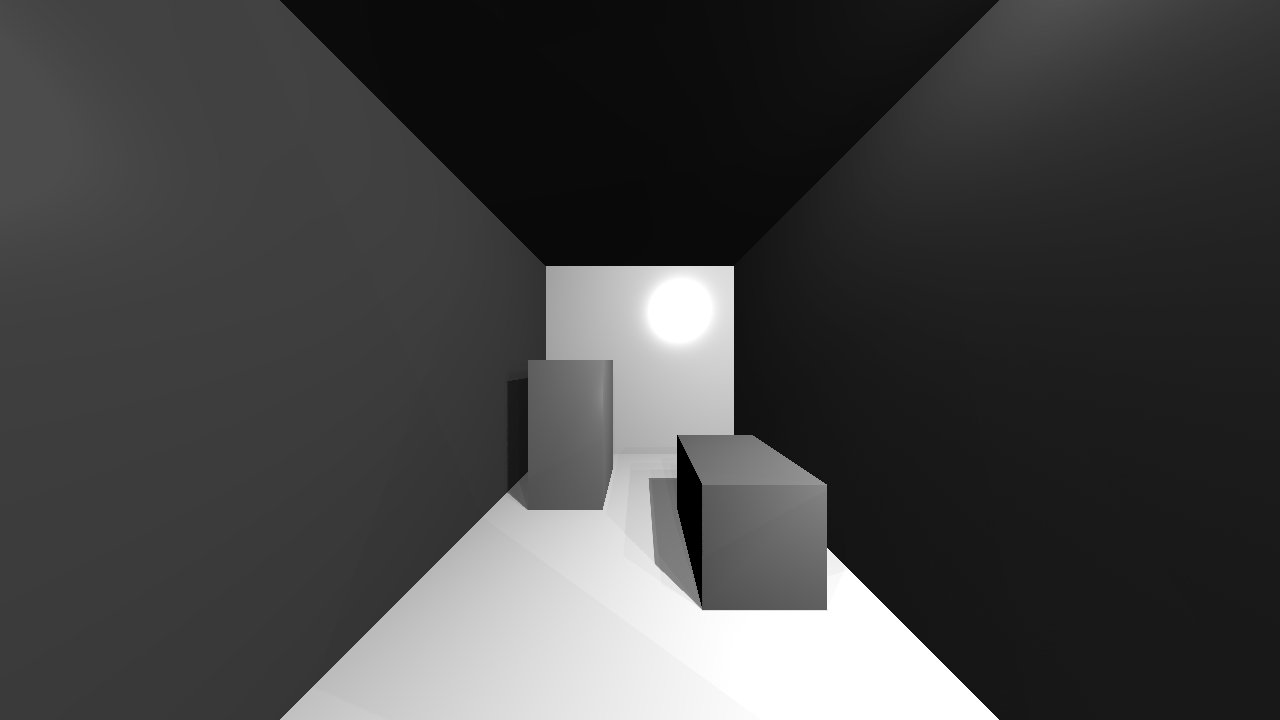
\includegraphics[width=\textwidth]{sample4_gray.jpg}
                \caption{Light is at the near upper right corner of the scene.}
                \label{fig:sample4}
        \end{subfigure}
        \begin{subfigure}[b]{0.5\textwidth}
                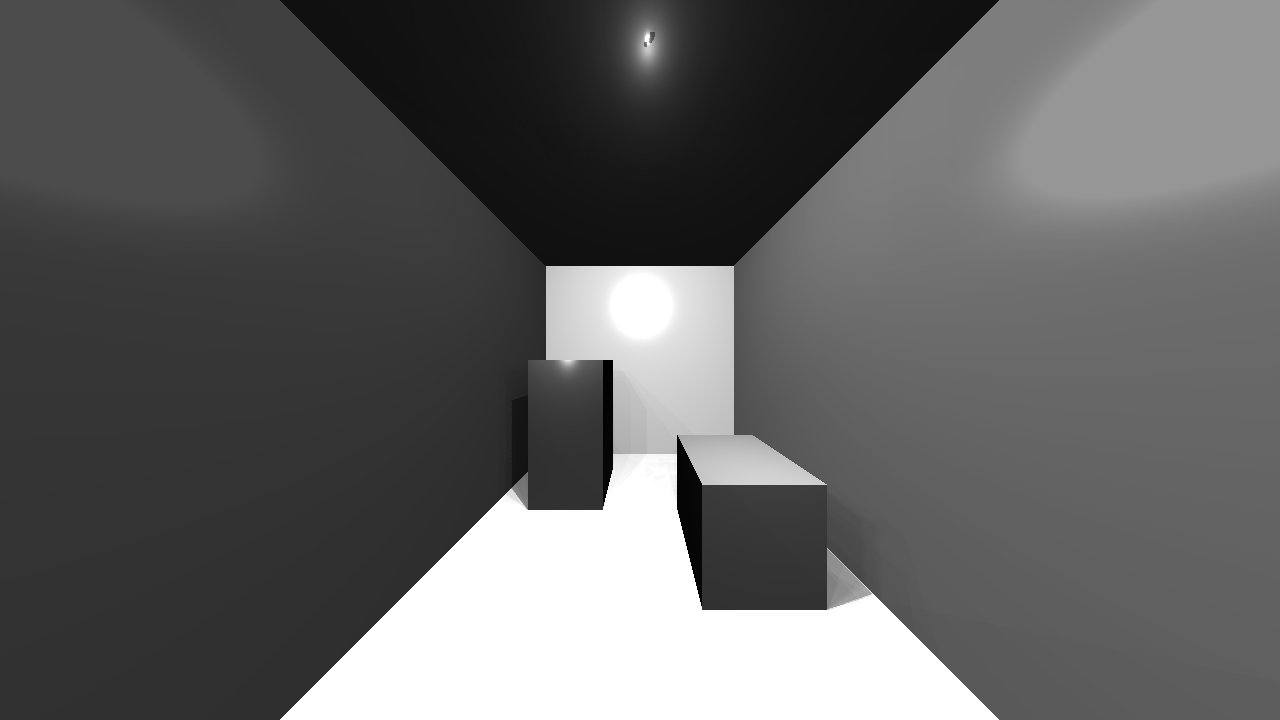
\includegraphics[width=\textwidth]{sample5_gray.jpg}
                \caption{Light is in the upper center of the scene.}
                \label{fig:sample5}
        \end{subfigure}
        \caption{Additional Rendered Images Using the Default Parameters}\label{fig:default}
\end{figure}


\chapter{CONCLUSION}

\section{General Observations}
\paragraph{}
Most importantly, indirect shadows are an expensive luxury.  They can require a lot of GPU memory and a lot of computing power depending on the approach.  If accurate indirect shadows are a must, a lot of GPU memory must be available in order to make the shadows look good.  This is due in part to the need to have the shadow maps be large.  They must be large enough compared to the screen size in order to minimize the amount of jaggies on edges of the shadows.  For this implementation, three times larger than the screen size appeared to be best, but just like all of the other parameters of this method, this factor can be changed.  As computing technology advances further, more GPU's will have more memory available and will then be able to support more shadow maps of larger size, but in the meantime, in order to get more realistic looking images, it is best to approximate indirect shadows.

\paragraph{}
As mentioned in section \ref{sec:study}, due to the low frequency nature of indirect shadows, accurate visibility is not required.  Also in that study, imperfect shadows were considered the most realistic of the approximated methods.  Therefore, the use of integrated shadows as discussed in section \ref{sec:newApproach} performed better than accurate shadows and due to the shadow limitations of using accurate shadows looked more realistic.  These shadows appeared more realistic due to being smoother and less segregated than the accurate visibility shadows reinforcing the notion that smoother inaccurate shadows look more realistic than segregated accurate shadows.  By using these shadows, the Light Wave method is more scalable in terms of portability to different types of machines with different computing capabilities as well as more scalable when it comes to increased scene complexity.

\section{Implementation Specific Final Thoughts}
\paragraph{}
Light Wave is a technique of estimating the indirect lighting in a scene in real-time.  It is able to do this through the use of virtual point lights or VPL's structured outward from the primary light source in such a way so that the direct light can wrap around objects and hit surfaces that may not be directly visible from the primary light source.  These VPL's are structured in hemispheres around the primary light source with extended viewing capabilities.  These attributes make the overall flow of the light in the scene to resemble a wave flowing outward from the primary light source in all directions and wrapping around obscuring objects.  Therefore, we approximate indirect lighting using only direct lighting calculations from upwards of thousands of light sources.  We are only concerned with where each light ray terminates and not what happens afterwards thus simplifying the calculation.  By doing this we avoid the infinite number of iterations from using a Neumann series to calculate the infinite bouncing of light throughout a scene.

\paragraph{}
An aim of Light Wave is that it can be scalable.  The implementation allows for the adjustment of parameters to allow the user to increase/decrease performance and thus decrease/increase quality depending on the computing power available and required quality.  The implementation will also allow for more accurate renderings provided computing advancements.  The default parameter implementation using accurate shadows as detailed in prior sections leads to 55 frames per second with a simple scene and after reducing VPL count runs a complex scene at 26 FPS on the current machine (see section \ref{sec:impdetails} for specifics).  It is assumed that some machines will perform slower than ours, therefore, we provided some suggestions on how to modify the parameters in order to maximize performance with limited quality impact in section \ref{sec:finalAnalysis}.  For machines that can handle the defaults and crave more realistic renderings, the first thing to increase would be the number of indirect shadow maps to smooth out the indirect shadows.

\paragraph{}
When using integrated shadows, we were able to render many more shadows than when using accurate shadows at similar FPS.  For example, we could render 60 integrated shadows at 60FPS while we could render 20 accurate shadows at 55FPS.  Integrated shadows also scaled better with an increase in scene complexity.  After similarly reducing the VPL count as with the accurate shadows, while using integrated shadows we were able to render 120 indirect shadows on the most complicated scene at 30FPS as opposed to 20 indirect shadows at 26FPS when using accurate shadows.  See tables \ref{table:tech1Complex} and \ref{table:tech2Complex} for details.  For machines that can handle more, the first thing to increase could be either the number of indirect shadow maps or the number of steps for the integrated shadows to render even more shadows.

\paragraph{}
Therefore, this implementation was successful in it's goal of approximating indirect illumination in real-time using the GPU.  It achieves fairly realistic rendered scenes that are fully dynamic allowing the user to move objects and the light in real-time.  It also proves portable with adjustable parameters allowing it to scale to the computing capabilities of the current machine as well as the complexity of the scene.  It also provides two different types of shadowing techniques using either accurate or integrated shadows.  Future advances in computing power would allow for specific changes in parameters to allow for more realistic renderings.  These include the use of additional VPL's, use of higher resolutions, use of additional indirect shadow maps for either shadowing technique, or additional steps for the integrated shadows technique in order to render ultra-realistic indirect shadows.

\section{Limitations}
\paragraph{}
Light Wave's limitations include some of the same problems encountered in other VPL-driven techniques.  This primarily includes singularities due to the VPL contributions coming from a single discrete location.  A limitation when using accurate shadows is that the number of indirect shadows drastically impacts performance due to the use of accurate visibility and the maximum number of shadow maps is limited by the amount of GPU memory available.  Integrated shadows can be used instead in order to limit GPU memory required and increase the realism of the indirect shadows.  Lastly, in order to keep the scene fully dynamic with full indirect shadows, VPL count needs to be lowered when scene complexity rises, but this can be done by increasing the VPL ray angle with limited impact on the resulting quality.

\section{Improvements}
\paragraph{}
Apart from the technological advances that would improve Light Wave's results, an interesting improvement that could be made to the technique would be to incorporate the idea of virtual ray lights Novák et al. (2012) to remove the VPL singularities.  However, keeping with the spirit of waves, we could have each VPL be a virtual semicircle light or arc on the VPL hemisphere.  So instead of integrating each VPL on a straight line, each VPL would be integrated along this semicircle or arc removing singularities and likely reducing the number of VPL's needed to achieve adequate coverage of the scene as well as expanding the use of light waves.  Shadow map memory could be minimized using some texture compression approaches since neighboring entries are likely to be similar and approximations have been shown to be sufficient.  The shadow map resolution can be varied across the scene with increased resolution where depths vary greatly and reduced resolution where depths are similar.  Additional improvements could include the matrix sampling techniques of Hašan (2007), Ou and Pellacini (2011), or Walter et al. (2005) that would allow higher VPL numbers as well as using neighborhood optimizations found in Dachsbacher and Stamminger (2006) to increase performance.

% If you have appendices start it here. Make sure you have the file "appenda.tex" ready
% You can include more appendices
%\appendix
%\include{appenda}

% Let's start the bibliography - We are using bibtex.
% Make sure you have the file "thesis.bbl" ready
% If you are good at LaTex, you can generate this file using bibtex

\bibliography{references}

%
%
% All done.  Tell LaTeX bye-bye and graduate!
\end{document}
